\documentclass[12pt,a4paper,oneside]{book}

% --- Setting up a language ---

\usepackage[utf8]{inputenc}
\usepackage[english,main=ukrainian]{babel}

% --- Detault Packages ---

\usepackage[dvipsnames]{xcolor}

\usepackage[toc,page]{appendix}
\usepackage{amsthm,amsfonts,mathtools,amscd,amssymb,mathrsfs}
\usepackage{latexsym}
\usepackage{euscript}
\usepackage{multicol}
\usepackage{bbm}
\usepackage{pgffor}   % For loops in TikZ
\usepackage{dsfont}
\usepackage{pgfplots}
\usepackage{graphicx}
\usepackage{tikz}
\usetikzlibrary{backgrounds}
\usepackage{array}
\usepackage{caption}
\usepackage{subcaption}
\usepackage{listings}
\usepackage{setspace}
\usepackage[shortlabels]{enumitem}

% 
\usepackage[unicode]{hyperref}
\hypersetup{colorlinks=true}
\tolerance=9000 
\textwidth=165mm
\textheight=250mm 
\oddsidemargin=4.6mm
\voffset=-20mm
\binoppenalty=1 \relpenalty=1 
\allowdisplaybreaks
\everymath{\displaystyle}
\renewcommand{\baselinestretch}{1.44}

\usepackage{dipl}
\pagestyle{headings}
\graphicspath{ {figures/} }

% --- Theorem Styles ---
\theoremstyle{dplplain}
\newtheorem{theorem}{Теорема}[chapter]
\newtheorem{corollary}[theorem]{Наслідок}%[chapter]
\newtheorem{statement}[theorem]{Твердження}%[chapter]
\newtheorem{lemma}[theorem]{Лема}%[chapter]
\theoremstyle{dpldefinition}
\newtheorem{definition}[theorem]{Означення}%[chapter]
\theoremstyle{dplremark}
\newtheorem{problem}[theorem]{Задача}%[chapter]
\newtheorem{remark}[theorem]{Зауваження}%[chapter]
\newtheorem{example}[theorem]{Приклад}%[chapter]

% --- Math shortings ---
\DeclareMathOperator*{\esssup}{ess\,sup}
\DeclareMathOperator*{\essinf}{ess\,inf}
\DeclareMathOperator*{\bigtimes}{\mbox{\raisebox{-0.5ex}{\huge$\times$}}}
\DeclareMathOperator*{\smalltimes}{\mbox{\raisebox{-0.3ex}{\large$\times$}}}
\DeclareMathOperator*{\ootimes}{\overline{\otimes}}

\DeclareMathOperator*{\argmax}{arg\,max}
\DeclareMathOperator*{\argmin}{arg\,min}

% --- Listings ---
% --- Default settings ---
% \lstset{language=Python}
% \lstset{frame=lines}
% \lstset{basicstyle=\normalsize}
% \lstset{prebreak=\raisebox{-2ex}[0ex][0ex]{\ensuremath{\hookleftarrow}}}
% \lstset{breaklines=true}
% \captionsetup[lstlisting]{font=large}

% --- My own settings ---
\definecolor{dkgreen}{rgb}{0,0.5,0}
\definecolor{gray}{rgb}{0.5,0.5,0.5}
\definecolor{mauve}{rgb}{0.58,0,0.82}
\lstset{
    numbers=left,  
    frame=tb,
    aboveskip=3mm,
    belowskip=3mm,
    showstringspaces=false,
    columns=fixed,
    framerule=1pt,
    rulecolor=\color{gray!35},
    backgroundcolor=\color{gray!5},
    basicstyle={\ttfamily\small},
    numberstyle=\footnotesize\color{gray},
    keywordstyle=\bfseries\color{MidnightBlue!95!black},
    commentstyle=\color{dkgreen},
    stringstyle=\color{mauve},
    breaklines=true,
    breakatwhitespace=true,
    tabsize=2,
    extendedchars=false,
    postbreak=\mbox{\hspace{-1.4em}\textcolor{purple}{$\hookrightarrow$}\space}
}

\newcommand{\remind}[1]{\textcolor{red}{\textbf{#1}}} % To remind me of unfinished work to fix later
\newcommand{\hide}[1]{} % To hide large blocks of code without using % symbols


% --- Bibliography ---
\usepackage[
    backend=biber,
    style=alphabetic
]{biblatex}
\addbibresource{main.bib}

\begin{document}
%%%%%%%%%%%%%%%%%%%%%%%%%%%%%%%%%%%%%%%%%%%%%%%
%%%%%%%%%%%%% вибір титульної сторінки %%%%%%
%
% Для правильного оформлення роботи 
% треба вибрати титульну сторінку. 
%
% Для студентів 4 курсу треба 
% прибрати знак відсотку (%)
% перед командою \begin{titlepage}
	\setstretch{1}
	\begin{center}
		\Large Харківський національний університет імені В.Н.~Каразіна\\
		Факультет математики і інформатики\\
		Кафедра прикладної математики
	\end{center}

	\vfill
		
	\begin{center}	
		\LARGE \bfseries Навчально-виробнича практика
		% \\
		% 	{\normalsize \mdseries освітньо-кваліфікаційний рівень: \bfseries \slshape бакалавр}
		\\[0.5\baselineskip]
		{\mdseries на тему} \bfseries\slshape <<Activation-Efficient Neural Network Architectures>> \\[0.5\baselineskip]
	\end{center}
	
	\vfill
	

	\setlength{\tabcolsep}{3pt}
	\hbox to \textwidth{\hfill\begin{tabular}{>{\slshape}lp{0.43\textwidth}}
			Виконав: &студент групи МП41 IV курсу
			
			(перший бакалаврський рівень), 
			
			спеціальності 113 
			
			``Прикладна математика''
			
			освітньої програми 
			
			``Прикладна математика''
			
			\textbf{Захаров~Д.О.}
			\\[0.5\baselineskip]
			Керівник: & доктор фіз.-мат. наук, 
			
			професор кафедри 
			
			прикладної математики
			
			\textbf{Ігнатович С.Ю.}	
			% \\[0.5\baselineskip]
			% Рецензент: & кандидат фіз.-мат. наук, 
			
			% доцент кафедри 
			
			% прикладної математики
			
			% \textbf{Хтось.}
	\end{tabular}	}
	
\vspace{\baselineskip}
	
	\begin{center}
		Харків --- 2025 рік
	\end{center}
	
\end{titlepage} 
% при цьому перед іншими двома командами 
% мають стояти знаки відсотку (%).
% 
% Для студентів 6 курсу ОПП треба 
% прибрати знак відсотку (%)
% перед командою \begin{titlepage}
	\setstretch{1}
	\begin{center}
		\Large Харківський національний університет імені В.Н.~Каразіна\\
		Факультет математики і інформатики\\
		Кафедра прикладної математики
	\end{center}

	\vfill
		
	\begin{center}	
		\LARGE \bfseries Кваліфікаційна робота
		\\
			{\normalsize \mdseries освітньо-кваліфікаційний рівень: \bfseries \slshape магістр}
		\\[0.5\baselineskip]
		{\mdseries на тему} \bfseries\slshape <<Класи множин>> \\[0.5\baselineskip]
	\end{center}
	
	\vfill
	

	\setlength{\tabcolsep}{3pt}
	\hbox to \textwidth{\hfill\begin{tabular}{>{\slshape}lp{0.42\textwidth}}
			Виконав: &студент групи МП62 VI курсу
			
			(другий магістерський рівень), 
			
			спеціальності 113 
			
			``Прикладна математика''
			
			освітньо-професійної програми 
			
			``Прикладна математика''
			
			\textbf{Петренко~І.В.}
			\\[0.5\baselineskip]
			Керівник: & доктор фіз.-мат. наук, 
			
			професор кафедри 
			
			прикладної математики
			
			\textbf{Іваненко П.К.}	
			\\[0.5\baselineskip]
			Рецензент: & кандидат фіз.-мат. наук, 
			
			доцент кафедри 
			
			прикладної математики
			
			\textbf{Стеценко М.В.}
	\end{tabular}	}
	
\vspace{\baselineskip}
	
	\begin{center}
		Харків --- 2023 рік
	\end{center}
	
\end{titlepage} 
% при цьому перед іншими двома командами 
% мають стояти знаки відсотку (%).
% 
% Для студентів 6 курсу ОНП треба 
% прибрати знак відсотку (%)
% перед командою \begin{titlepage}
	\setstretch{1}
	\begin{center}
		\Large Харківський національний університет імені В.Н.~Каразіна\\
		Факультет математики і інформатики\\
		Кафедра прикладної математики
	\end{center}

	\vfill
		
	\begin{center}	
		\LARGE \bfseries Курсова науково-дослідницька робота
		\\
			{\normalsize \mdseries освітньо-кваліфікаційний рівень: \bfseries \slshape магістр}
		\\[0.5\baselineskip]
		{\mdseries на тему} \bfseries\slshape <<Класи множин>> \\[0.5\baselineskip]
	\end{center}
	
	\vfill
	

	\setlength{\tabcolsep}{3pt}
	\hbox to \textwidth{\hfill\begin{tabular}{>{\slshape}lp{0.42\textwidth}}
			Виконав: &студент групи МП61 VI курсу
			
			(другий магістерський рівень), 
			
			спеціальності 113 
			
			``Прикладна математика''
			
			освітньо-наукової програми 
			
			``Прикладна математика''
			
			\textbf{Петренко~І.В.}
			\\[0.5\baselineskip]
			Керівник: & доктор фіз.-мат. наук, 
			
			професор кафедри 
			
			прикладної математики
			
			\textbf{Іваненко П.К.}	
			\\[0.5\baselineskip]
			Рецензент: & кандидат фіз.-мат. наук, 
			
			доцент кафедри 
			
			прикладної математики
			
			\textbf{Стеценко М.В.}
	\end{tabular}	}
	
\vspace{\baselineskip}
	
	\begin{center}
		Харків --- 2024 рік
	\end{center}
	
\end{titlepage} 
% при цьому перед іншими двома командами 
% мають стояти знаки відсотку (%).
%
%%%%%%%%%%%%%%%%%%%%%%%%%%%%%%%%%%%%%%%%

\begin{titlepage}
	\setstretch{1}
	\begin{center}
		\Large Харківський національний університет імені В.Н.~Каразіна\\
		Факультет математики і інформатики\\
		Кафедра прикладної математики
	\end{center}

	\vfill
		
	\begin{center}	
		\LARGE \bfseries Навчально-виробнича практика
		% \\
		% 	{\normalsize \mdseries освітньо-кваліфікаційний рівень: \bfseries \slshape бакалавр}
		\\[0.5\baselineskip]
		{\mdseries на тему} \bfseries\slshape <<Activation-Efficient Neural Network Architectures>> \\[0.5\baselineskip]
	\end{center}
	
	\vfill
	

	\setlength{\tabcolsep}{3pt}
	\hbox to \textwidth{\hfill\begin{tabular}{>{\slshape}lp{0.43\textwidth}}
			Виконав: &студент групи МП41 IV курсу
			
			(перший бакалаврський рівень), 
			
			спеціальності 113 
			
			``Прикладна математика''
			
			освітньої програми 
			
			``Прикладна математика''
			
			\textbf{Захаров~Д.О.}
			\\[0.5\baselineskip]
			Керівник: & доктор фіз.-мат. наук, 
			
			професор кафедри 
			
			прикладної математики
			
			\textbf{Ігнатович С.Ю.}	
			% \\[0.5\baselineskip]
			% Рецензент: & кандидат фіз.-мат. наук, 
			
			% доцент кафедри 
			
			% прикладної математики
			
			% \textbf{Хтось.}
	\end{tabular}	}
	
\vspace{\baselineskip}
	
	\begin{center}
		Харків --- 2025 рік
	\end{center}
	
\end{titlepage}

%\begin{titlepage}
	\setstretch{1}
	\begin{center}
		\Large Харківський національний університет імені В.Н.~Каразіна\\
		Факультет математики і інформатики\\
		Кафедра прикладної математики
	\end{center}

	\vfill
		
	\begin{center}	
		\LARGE \bfseries Кваліфікаційна робота
		\\
			{\normalsize \mdseries освітньо-кваліфікаційний рівень: \bfseries \slshape магістр}
		\\[0.5\baselineskip]
		{\mdseries на тему} \bfseries\slshape <<Класи множин>> \\[0.5\baselineskip]
	\end{center}
	
	\vfill
	

	\setlength{\tabcolsep}{3pt}
	\hbox to \textwidth{\hfill\begin{tabular}{>{\slshape}lp{0.42\textwidth}}
			Виконав: &студент групи МП62 VI курсу
			
			(другий магістерський рівень), 
			
			спеціальності 113 
			
			``Прикладна математика''
			
			освітньо-професійної програми 
			
			``Прикладна математика''
			
			\textbf{Петренко~І.В.}
			\\[0.5\baselineskip]
			Керівник: & доктор фіз.-мат. наук, 
			
			професор кафедри 
			
			прикладної математики
			
			\textbf{Іваненко П.К.}	
			\\[0.5\baselineskip]
			Рецензент: & кандидат фіз.-мат. наук, 
			
			доцент кафедри 
			
			прикладної математики
			
			\textbf{Стеценко М.В.}
	\end{tabular}	}
	
\vspace{\baselineskip}
	
	\begin{center}
		Харків --- 2023 рік
	\end{center}
	
\end{titlepage}

%\begin{titlepage}
	\setstretch{1}
	\begin{center}
		\Large Харківський національний університет імені В.Н.~Каразіна\\
		Факультет математики і інформатики\\
		Кафедра прикладної математики
	\end{center}

	\vfill
		
	\begin{center}	
		\LARGE \bfseries Курсова науково-дослідницька робота
		\\
			{\normalsize \mdseries освітньо-кваліфікаційний рівень: \bfseries \slshape магістр}
		\\[0.5\baselineskip]
		{\mdseries на тему} \bfseries\slshape <<Класи множин>> \\[0.5\baselineskip]
	\end{center}
	
	\vfill
	

	\setlength{\tabcolsep}{3pt}
	\hbox to \textwidth{\hfill\begin{tabular}{>{\slshape}lp{0.42\textwidth}}
			Виконав: &студент групи МП61 VI курсу
			
			(другий магістерський рівень), 
			
			спеціальності 113 
			
			``Прикладна математика''
			
			освітньо-наукової програми 
			
			``Прикладна математика''
			
			\textbf{Петренко~І.В.}
			\\[0.5\baselineskip]
			Керівник: & доктор фіз.-мат. наук, 
			
			професор кафедри 
			
			прикладної математики
			
			\textbf{Іваненко П.К.}	
			\\[0.5\baselineskip]
			Рецензент: & кандидат фіз.-мат. наук, 
			
			доцент кафедри 
			
			прикладної математики
			
			\textbf{Стеценко М.В.}
	\end{tabular}	}
	
\vspace{\baselineskip}
	
	\begin{center}
		Харків --- 2024 рік
	\end{center}
	
\end{titlepage}

%%%% кінець вибору титульної сторінки %%%%%%

\refstepcounter{page}

\chapter*{Анотації}
\markboth{Анотації}{Анотації}
\addcontentsline{toc}{chapter}{Анотації}

\subsubsection{Захаров Д.О. Математичні основи штучних нейронних мереж.}

В сучасному світі важко уявити сферу, де б не використовувались штучні нейронні
мережі. Проте, незважаючи на таку кількість різноманітних досліджень, більшість
з них не обгрунтовують чому саме нейронні мережі так добре апроксимують данні та
видають гарну точність. Ця робота призначена опису фундаменту нейронних мереж
та, в певній мірі, формалізації процесу навчання: що саме розв'язують нейронні
мережі, чому вони (теоретично) здатні апроксимувати важливі для нас залежності і
як на практиці реалізувати процес підбору параметрів моделі.

\subsubsection{Zakharov D.O. Mathematical foundations of artificial neural networks.}

In the modern world, it is almost impossible to imagine a technical field 
where artificial neural networks are not used. However, despite the abundance
of research of their applications, most of them do not explain why neural networks
are so good at approximating data and achieving high accuracy. This work is
dedicated to describing the fundamentals of neural networks and, to some extent,
formalizing the learning process: what neural networks solve, why they are
(theoretically) capable of approximating important dependencies, and how to
practically implement the process of selecting model parameters.


\tableofcontents

\chapter*{Вступ}
\markboth{Вступ}{Вступ}
\addcontentsline{toc}{chapter}{Вступ}

Без всяких сумнівів, нейронні мережі є одними з найбільш популярних інструментів
машинного навчання для пошуку складних залежностей. Вони використовуються в
безлічі різних областей, таких як комп'ютерний зір \cite{cv-survey}, обробка
природних мов \cite{nlp-survey} та біометричних данних \cite{biometrics-survey},
розробка рекомендаційних систем \cite{recommendation-systems-survey}, генерації
зображень \cite{gan-survey} тощо. Наші нещодавні дослідження
\cite{our-biometrics-1,our-biometrics-2,our-biometrics-3} додатково підтвердили
високу ефективність нейронних мереж у задачах кібербезпеки та систем захисту
біометричних даних. Що уж там, мабуть кожна людина чула або використовувала
новітні розробки OpenAI --- архітектуру \textit{GPT-3} (Generative Pre-trained
Transformer) \cite{chatgpt} або \textit{Open AI o1}, що вже навіть здатна
розв'язувати задачі з міжнародної олімпіади з математики або аналізувати складні
наукові тексти. 

Проте, незважаючи на таку кількість різноманітних досліджень, більшість з них 
зводиться до доволі типічного алгоритму (звичайно, з варіаціями в залежності від
конкретної задачі):
\begin{enumerate}
    \item Визначення типу задачі (класифікація, регресія, сегментація, тощо).
    \item Підбір набору даних (далі, скорочено --- датасет).
    \item Вибір архітектури моделі, функції втрати та метрик якості.
    \item Тренування та корегування параметрів моделі для максимізації метрики якості.
    \item Аналіз результатів.
\end{enumerate}

Проте, протягом цього процесу, ми зазвичай пропускаємо одне доволі
фундаментальне питання: а чому, взагалі кажучи, обрані архітектури нейронних
мереж здатні вирішувати такі задачі? Звичайно, що для практичних задач це
питання часто не принципове: якщо воно працює і працює добре, то цього більш,
ніж достатньо\footnote{Тим не менш, в сучасних роботах іноді трапляється спроба
пояснити, чому описана методологія може теоретично дати, скажімо, мінімум для
певної метрики, як це було зроблено в оригінальному описі генеративних
адверсальних мереж (Generative Adversarial Networks) \cite{gan}}.

Саме тому ми присвятили цю роботу опису фундаменту нейронних
мереж та, в певній мірі, формалізації процесу навчання: що саме 
розв'язують нейронні мережі, чому вони (теоретично) здатні
апроксимувати важливі для нас залежності і як на практиці
реалізувати процес підбору параметрів моделі.



\usetikzlibrary{positioning, arrows.meta}

\chapter{Задачі машинного навчання}

\section{Що таке модель?}

Насправді, чітко поставити задачу сучасної теорії машинного навчання одним
визначенням дуже складно. Це пов'язано з тим, що підхід до розв'язку задачі дуже
залежить від того, що ми очікуємо від так званої \textit{моделі машинного
навчання}. Що ж ми розуміємо під терміном ``модель''?

Найчастіше, на вхід подається певний набір данних $\mathcal{D}$. Це можуть бути
картинки разом з маркуванням, що зображено. Можуть бути текстові данні, чисельні
данні, аудіо- або відео-записи, результати вимірювань на сенсорних пристроях,
тощо. Маючи цей набір даних, ми часто хочемо зрозуміти певні закономірності в
цих даних. Функцію, що бере певний вхід, що містить інформацію про об'єкт, і
повертає вихід, що містить закономірність, часто називаємий
\textit{передбаченням}, як раз і називають \textbf{моделлю}. Далі наведемо
кілька нетривільних прикладів з задач машинного навчання.

\begin{example}[Класифікація цифр]
	Будь-яке сіро-біле зображення $\boldsymbol{X}$ розміру $W \times H$ пікселів
	можна розглядати як матрицю $\boldsymbol{X} \in \mathbb{R}^{W \times H}$, де
	кожен елемент матриці $X_{i,j}$ --- це значення яскравості відповідного
	пікселя на позиції $(i,j)$ (наприклад, значення $0$ може позначати чорний
	колір, $1$ --- білий, а значення проміж --- степінь сірості)\footnote{Іноді
	таку множину явно записують як $[0,1]^{W \times H}$, щоб підкреслити, що
	значення нормалізовані на відрізок $[0,1]$. Тим не менш, використовуємо
	позначення $\mathbb{R}^{W \times H}$, оскільки оптимальна нормалізація
	данних залежить від обраної методології}. 
	
	Нехай нам наданий набір $\mathcal{D} =
	\{(\boldsymbol{X}_n,y_n)\}_{1 \leq n \leq N}$ --- пари
	``зображення-цифра'', де $y_n \in \{0,\dots,9\}$. Наша ціль ---
	побудувати так звану \textit{класифікаційну модель} $f: \mathbb{R}^{W \times
	H} \to \{0,\dots,9\}$, яка буде приймати на вхід зображення
	$\boldsymbol{X}$ та видавати цифру $f(\boldsymbol{X})$, що зображена.
	Приклад зображено на Рисунку~\ref{fig:digits} на базі набору данних MNIST
	\cite{mnist}.

	\begin{figure}
		\centering
		\begin{tikzpicture}
			% Define grid and spacing size
			\def\gridsize{3}
			\def\xspacing{4} % Horizontal spacing
			\def\yspacing{3} % Vertical spacing
			
			% Loop to create 3x3 grid with predictions
			\foreach \row in {1,2,3} {
				\foreach \col in {1,2,3} {
			
					% Calculate image index for sample prediction (0-9, can be random or set)
					\pgfmathtruncatemacro{\digitindex}{(\row-1)*\gridsize + \col - 1}

					% Placeholder integer predictions (customize as needed)
					\pgfmathtruncatemacro{\prediction}{mod(\digitindex, 10)} % Dummy prediction for illustration
					
					% Position of each MNIST image
					\node[draw, minimum size=1cm, inner sep=0pt] (img\row\col) at (\col*\xspacing, -\row*\yspacing)
					{\includegraphics[width=1.75cm]{figures/mnist/digit\digitindex.png}};
			
					% Prediction label with actual prediction value next to each digit
					\node[right=1.0cm of img\row\col] (pred\row\col) {\textbf{\prediction}};
			
					% Arrow pointing from image to prediction
					\draw[->, thick] (img\row\col) -- node[above] {\( f \)} (pred\row\col);
				}
			}
		\end{tikzpicture}
		\caption{Приклад класифікації цифр. Маючи зображення $X \in \mathbb{R}^{W \times H}$, наша функція дає дискретне передбачення $f(X) \in \{0,\dots,9\}$ --- цифра, яка зображена на зображенні $X$.}
		\label{fig:digits}
	\end{figure}

\end{example}

\begin{example}[Розпізнавання дрону]
	Нехай наша задача: це розпізнати розташування дронів на кадрі відео. Нехай в
	нас кольорове зображення розміру $W \times H$. Тоді зображення
	$\boldsymbol{X}$ береться з множини $\mathbb{R}^{W \times H \times 3}$,
	де замість яскравості пікселя, маємо тривимірний вектор $(r,g,b) \in
	\mathbb{R}^3$ --- колір пікселя (інтенсивність червоного, зеленого та синіх
	каналів, відповідно).

	Поділимо наше зображення на сітку розміру $n_W \times n_H$. Тоді в якості
	моделі можна взяти функцію $f: \mathbb{R}^{W \times H \times 3} \to
	\mathbb{R}^{n_W \times n_H}$, що видає матрицю
	$\{p(S_{i,j}|\boldsymbol{X})\}_{1 \leq i \leq n_W, \, 1 \leq j \leq n_H}$,
	де $S_{i,j}$ --- подія ``в клітинці $(i,j)$ сітки знаходиться дрон''. Ця
	модель візуально проілюстрована на Рис.~\ref{fig:drone}. Відмітимо, що ідея
	описаної конструкції частково використовується в архітектурі YOLO (You Look
	Only Once) \cite{yolo} --- одній з найпопулярніших архітектур для
	розпізнавання об'єктів на зображеннях.

	\begin{figure}
	
	\centering
	\begin{tikzpicture}

		% Set up background image
		\node[inner sep=0pt, anchor=center] at (0,0) {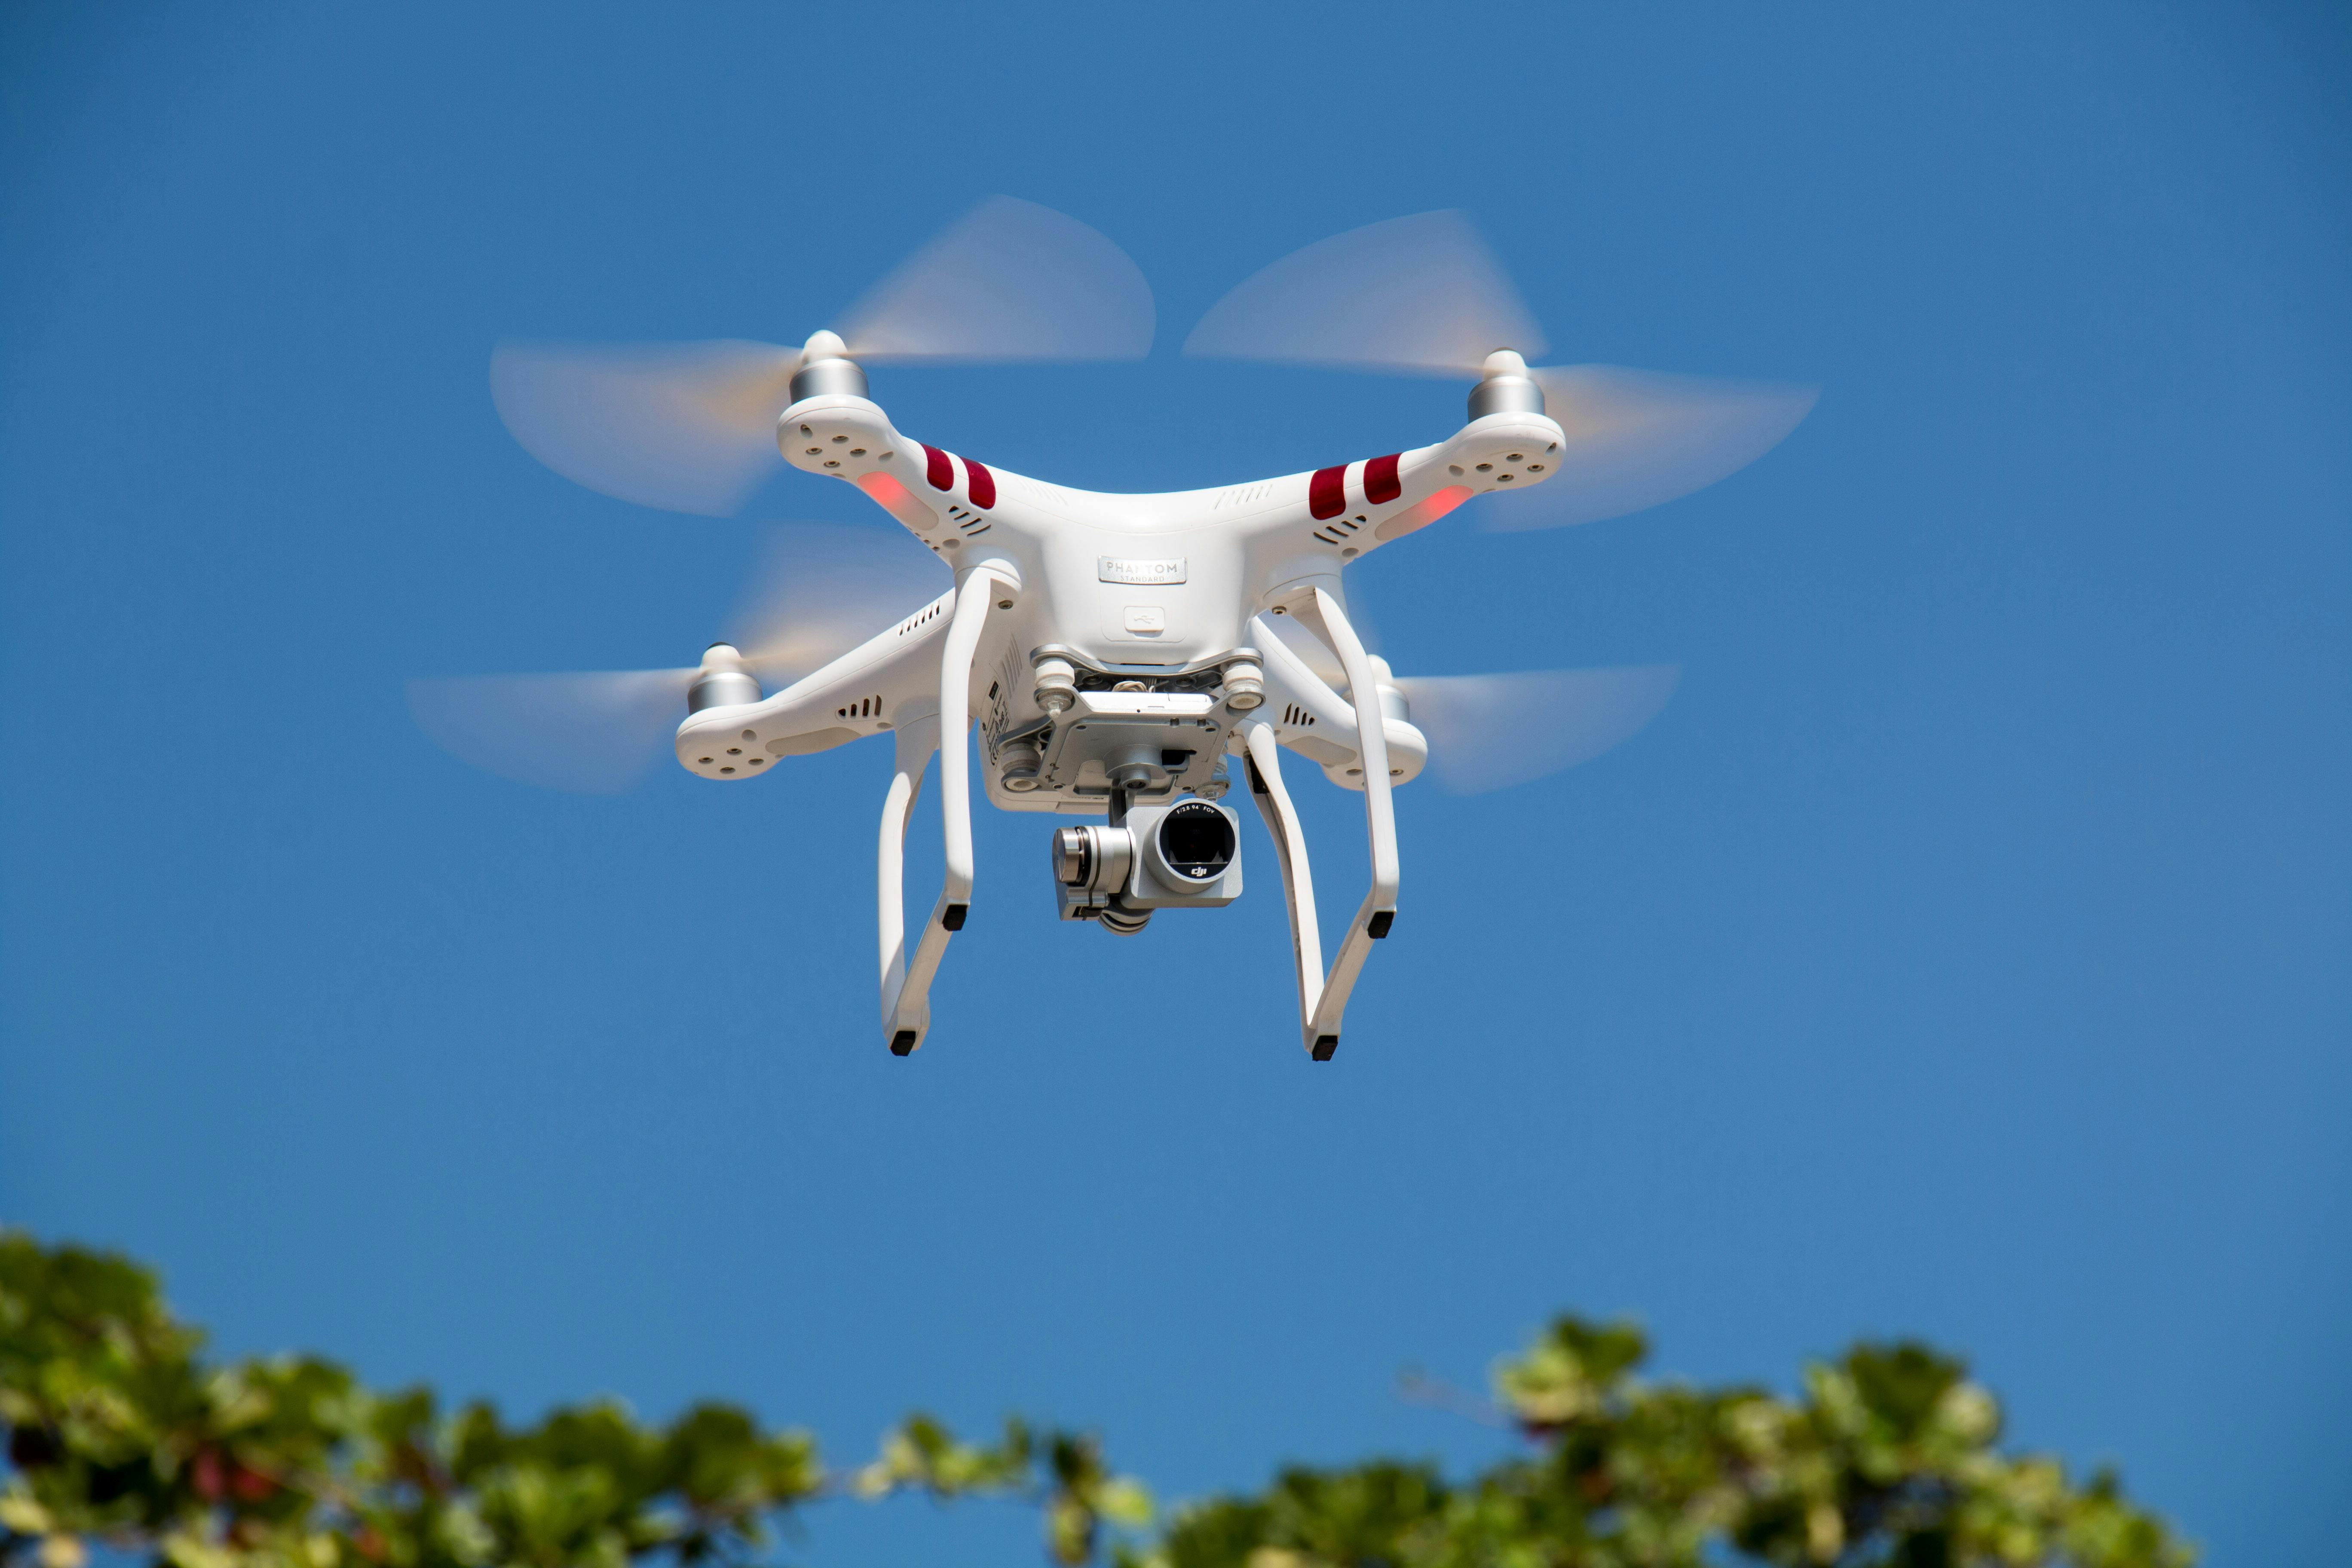
\includegraphics[width=10cm]{drone.jpg}}; % Replace 'background_image.jpg' with the path to your image
		
		% Define grid parameters
		\def\gridsize{7}
		\def\cellsize{1.5} % Size of each cell
		
		% Define the location of the object in the background (center of the image)
		\def\objectX{0} % X position of the object (centered in the image)
		\def\objectY{0} % Y position of the object (centered in the image)
		
		% Draw the gradient grid overlay with dashed borders
		\foreach \x in {-3,-2,-1,0,1,2} {
			\foreach \y in {-2,-1,0,1} {
				\definecolor{cellcolor}{rgb}{0.6, 0.8, 1} % Cold color (light blue)
				\ifnum\x=0\ifnum\y=0
					\definecolor{cellcolor}{rgb}{1, 0.6, 0.6} % Warm color (red/pink)
				\fi\fi
				\ifnum\x=-1\ifnum\y=0
					\definecolor{cellcolor}{rgb}{1, 0.6, 0.6} % Warm color (red/pink)
				\fi\fi
				\ifnum\x=-2\ifnum\y=0
					% Light yellow
					\definecolor{cellcolor}{rgb}{1, 1, 0.6}
				\fi\fi
				\ifnum\x=0\ifnum\y=-1
				\definecolor{cellcolor}{rgb}{1, 0.8, 0.4} % Intermediate warm (orange/yellow)
				\fi\fi
				\ifnum\x=-1\ifnum\y=-1
				\definecolor{cellcolor}{rgb}{1, 0.8, 0.4} % Intermediate warm (orange/yellow)
				\fi\fi

				% % Calculate distance from the object's location
				% \pgfmathsetmacro{\distance}{sqrt((\x - \objectX)^2 + (\y - \objectY)^2)}
		
				% % Set color based on distance to simulate probability heatmap
				% \ifdim \distance pt < 1.5pt
				% 	\definecolor{cellcolor}{rgb}{1, 0.6, 0.6} % Warm color (red/pink)
				% \else\ifdim \distance pt < 2.5pt
				% 	\definecolor{cellcolor}{rgb}{1, 0.8, 0.4} % Intermediate warm (orange/yellow)
				% \else
				% 	\definecolor{cellcolor}{rgb}{0.6, 0.8, 1} % Cold color (light blue)
				% \fi\fi
		
				% Overlay gradient cell with transparency
				\fill[cellcolor, opacity=0.5] (\x*\cellsize, \y*\cellsize) rectangle ++(\cellsize, \cellsize);
		
				% Draw dashed border around each cell
				\draw[line width=1pt, dashed] (\x*\cellsize, \y*\cellsize) rectangle ++(\cellsize, \cellsize);
			}
		}

		\draw[<-, ultra thick, bend right=90] (2.5,2) -- ++(3.0,-1) node[right] {$f_{1,5}(X) \approxeq 0.02$}; % Adjust coordinates for proper alignment
		\draw[<-, ultra thick, bend right=90] (0.5,-0.5) -- ++(6.0,-1) node[right] {$f_{3,4}(X) \approxeq 0.40$}; % Adjust coordinates for proper alignment

		\end{tikzpicture}
		\caption{Приклад розпізнавання дронів. Маючи зображення $\boldsymbol{X} \in \mathbb{R}^{W \times H \times 3}$, наша функція дає ймовірність того, що на кожному сегменті зображення знаходиться дрон. Чим тепліше кольори, тим вища ймовірність.}
		\label{fig:drone}
	\end{figure}
\end{example}

\begin{remark}
	Зверніть увагу, що в обох прикладах вище, модель $f$ видає дискретне або
	неперервне передбачення. Це може бути класифікація, регресія, сегментація,
	тощо. Це залежить від задачі, що ми розв'язуємо.
\end{remark}

\section{Параметризація моделей}
Проте, як саме ми будуємо моделі? Іншими словами, як обрати функцію $f$?
Зазвичай, ми маємо задати певне сімейство функцій $\mathcal{F}$, поміж яких ми
шукаємо ``найкращу''\footnote{Що таке ``найкраща'' функція, ми обговоримо
пізніше.} функцію. Наприклад, це може бути сімейство лінійних/квадратичних
функцій або функцій вигляду $f(x) = (\theta_1x^2, \theta_2 x)$. Звичайно,
оскільки алгоритм пошуку $f$ має бути заданий програмно, то ми не можемо
покласти в якості $\mathcal{F}$, скажімо, просто $L^2(\mathbb{R})$, бо тоді не
зрозуміло, як саме задати алгоритм пошуку $f$. Саме тому, для практичних
застосувань, ми \textit{параметризуємо} функції набором параметрів
$\boldsymbol{\theta}\in \Theta \subset \mathbb{R}^m$. Таким чином, наша модель
має вигляд $f(\mathbf{x}|\boldsymbol{\theta})$, де параметри
$\boldsymbol{\theta}$ можна змінювати, щоб зробити модель точною.

\begin{example}[Лінійна Регресія]
	Одна з класичних та найбільш відомих моделей --- це лінійна регресія. Нехай
	маємо набір даних $\mathcal{D} = \{(\mathbf{x}_n, y_n)\}_{1 \leq n \leq N}
	\subset \mathbb{R}^m \times \mathbb{R}$ і ми вважаємо, що залежність між
	$\mathbf{x}_n$ та $y_n$ лінійна. Іншими словами, ми введемо модель
	$f(\mathbf{x}|\boldsymbol{\theta}) = \boldsymbol{w}^{\top} \mathbf{x} +
	\beta$, де $\boldsymbol{\theta}=(\boldsymbol{w},\beta) \in \mathbb{R}^{m+1}$
	--- вектор параметрів. 

	В цілому, саме так дуже часто вводиться модель лінійної регресії. Проте, часто
	в літературі можна зустріти у якості моделі \textit{розподіл} величини $y$:
	\begin{equation}
		p(y|\mathbf{x},\boldsymbol{\theta}) = \mathcal{N}(y|\boldsymbol{w}^{\top}\mathbf{x} + \beta, \sigma^2),
	\end{equation}
	де $\boldsymbol{\theta} = (\boldsymbol{w},\beta,\sigma^2)$ --- вектор
	параметрів, а $\mathcal{N}(y|\mu,\sigma^2)$ --- щільність нормального
	розподілу. Така альтернатива дозволяє ввести більш гнучку модель, яка може
	давати степінь впевненості у своїх передбаченнях.
\end{example}

\begin{remark}
	Приклад вище легко узагальнити для випадку, коли вихід $\mathbf{y} \in \mathbb{R}^r$ --- вектор. В такому випадку, 
	моделлю є передбачення наступного розподілу:
	\begin{equation}
		p(\mathbf{y}|\mathbf{x},\boldsymbol{\theta}) = \prod_{i=1}^r \mathcal{N}(y_i|\boldsymbol{w}_i^{\top}\mathbf{x} + \beta_i, \sigma_i^2), \; \boldsymbol{w}_i \in \mathbb{R}^m, \; \beta_i,\sigma_i \in \mathbb{R}
	\end{equation}
\end{remark}

Отже, нехай ми вибрали параметризацію моделі. Як тепер обрати найкращі параметри?
Тут, наскільки б це не звучало банально, але знову все залежить від того, що ми
очікуємо від моделі:
\begin{itemize}
	\item Якщо наша модель має апроксимувати певну функцію $\varphi(\mathbf{x})$ на 
	обмеженій множині $\mathcal{X} \subset \mathbb{R}^r$, то ми можливо хочемо 
	мінімізувати $L^2(\mathcal{X},\mu)$ норму різниці:
	\begin{equation*}
		\hat{\boldsymbol{\theta}} = \argmin_{\boldsymbol{\theta} \in \Theta} \int_{\mathcal{X}} d\mu(\mathbf{x}) \left\| f(\mathbf{x}|\boldsymbol{\theta}) - \varphi(\mathbf{x}) \right\|_2^2
	\end{equation*}
	\item Можливо, ми хочемо максимізувати функцію правдоподібності:
	\begin{equation*}
		\hat{\boldsymbol{\theta}} = \argmax_{\boldsymbol{\theta} \in \Theta} \prod_{n=1}^N p(y_n|\mathbf{x}_n,\boldsymbol{\theta})
	\end{equation*}
	\item Якщо модель видає ймовірністний розподіл над простором $\Omega \subset \mathbb{R}^r$, то можливо ми хочемо мінімізувати відстань Кульбака-Лейблера до заданого розподілу $\pi(\mathbf{x})$:
	\begin{equation*}
		\hat{\boldsymbol{\theta}} = \argmin_{\boldsymbol{\theta} \in \Theta} D_{\mathbb{KL}}(f(\mathbf{x}|\boldsymbol{\theta})||\pi(\mathbf{x})) = \argmin_{\boldsymbol{\theta} \in \Theta} \int_{\Omega} f(\mathbf{x} | \boldsymbol{\theta}) \log \frac{f(\mathbf{x} | \boldsymbol{\theta})}{\pi(\mathbf{x})}d\mathbf{x}
	\end{equation*}
\end{itemize}

\begin{example}[Розв'язок лінійної регресії]
	Наприклад, нехай ми вирішуємо задачу лінійної регресії для набору даних
	$\mathcal{D} = \{(\mathbf{x}_n, y_n)\}_{1 \leq n \leq N}$. Нехай ми хочемо 
	мінімізовувати функцію правдоподібності:
	\begin{equation}
		\hat{\boldsymbol{\theta}} = \argmax_{\boldsymbol{\theta} \in \Theta} \prod_{n=1}^N p(y_n|\mathbf{x}_n,\boldsymbol{\theta}) = \argmax_{(\boldsymbol{w},\beta,\sigma^2)}\prod_{n=1}^N \mathcal{N}(y_n|\boldsymbol{w}^{\top}\mathbf{x}_n+\beta,\sigma^2)
	\end{equation}

	Можна довести, що якщо позначити $\mathbf{X} = [\mathbf{x}_1,\dots,\mathbf{x}_N] \in \mathbb{R}^{m \times N}$ --- матриця даних, а $\mathbf{y} = [y_1,\dots,y_N] \in \mathbb{R}^N$ --- вектор маркерів, то розв'язок має вигляд:
	\begin{equation}
		\hat{\boldsymbol{\theta}} = (\mathbf{X}\mathbf{X}^{\top})^{-1}\mathbf{X}\mathbf{y}
	\end{equation}
\end{example}

Проте, яку б ми теорію не використовували і які б параметризації моделей не
використовували, в кінці кінців, перед нами постає наступна задача оптимізації, що
розв'язується чисельно:
\begin{equation}
	\hat{\boldsymbol{\theta}} = \argmin_{\boldsymbol{\theta} \in \Theta} \mathcal{L}(\mathcal{D}|\boldsymbol{\theta}),
\end{equation}

де $\mathcal{L}(\mathcal{D}|\boldsymbol{\theta})$ --- функція втрат, яка
відображає як добре модель з параметрами $\boldsymbol{\theta}$ апроксимує дані
$\mathcal{D}$. Зауважимо, що хоч, в ідеалі, ми хочемо отримати вихід як
найближчий до ``істинного'', але в більшості випадків, ми не знаємо
``істинного'' вихідного розподілу. Тому, функція втрати, на практиці, 
залежить від набору данних $\mathcal{D}$, що подається на вхід, та від
параметризації $\boldsymbol{\theta}$.

Отже, стає питання: а як обрати параметризацію? Насправді, саме в цьому питанні
лежить більшість сучасних досліджень у глибокому навчанні: наприклад, у 1995
році, конволюційні нейронні мережі (Convolutional Neural Networks --- CNN)
прийшли на заміну повнозв'язним нейронним мережам \cite{lecun}, а механізм уваги
(Attention) у 2017 став основою багатьох NLP нейронних мереж \cite{attention}.
Щоб підкреслити важливість цього питання, наведемо приклад.

\begin{example}
	Нехай ми хочемо апроксимувати залежність $y(x)$ для набору $\mathcal{D} =
	\{(x_n,y_n)\}_{1 \leq n \leq N}$, причому навіть знаючи вибірку, ми не маємо
	уяви, яка має бути залежність $y(x)$. За невідомими причинами, нехай ми
	вирішили використати модель $f(x|\boldsymbol{\theta}) =
	\left(\sum_{i=1}^{1000}\theta_i\right)x$ для вектору параметрів
	$\boldsymbol{\theta} \in \mathbb{R}^{1000}$. Хоча ця модель містить досить
	велику кількість параметрів, вона не може апроксимувати жодні залежності
	окрім лінійних. Отже навіть якщо залежність $y$ від $x$ квадратична, що
	є відносно простою залежністю, модель не зможе її апроксимувати, незважаючи 
	на велику кількість параметрів.
\end{example}

\section{Основні задачі машинного навчання}

Отже, на практиці, ми хочемо мати як можна меньше параметрів, але при цьому 
модель повинна бути достатньо гнучкою, щоб апроксимувати будь-яку залежність. 
Інакшими слвоами, модель має апроксимувати як можна більш широкий клас 
функцій. 

Таким чином, підсумуємо, перед якими проблемами стоїть дослідник у глибокому
навчанні. Ми виділили три основні проблеми, які можна сформулювати наступним
чином: 
\begin{enumerate}
	\item \textbf{Проблема статистики/ймовірності/узагальнення:} маючи лише
	набір данних $\mathcal{D}$, не знаючи істинного розподілу чи функції, чи
	достатньо добре функція втрати $\mathcal{L}$ відображає степінь наближення
	моделі до істинної функції або розподілу?
	\item \textbf{Проблема оптимізації:} маючи функцію втрати $\mathcal{L}$,
	наскільки точно і чи взагалі можливо знайти оптимальні параметри
	$\boldsymbol{\theta}$ для мінімізації функції втрати?
	\item \textbf{Проблема апроксимації:} яка найкраща і чи взагалі існує така
	параметризація моделі, щоб вона була достатньо гнучкою, але при цьому мала
	якнайменшу кількість параметрів?\footnote{Мала кількість параметрів сприяє
	як і, очевидно, швидкості навчання та діставання передбачень, так і робить
	модель менш схильною до перенавчання та проблем градієнтів (стосується
	проблеми оптимізації).}
\end{enumerate}

В наступному підрозділі, ми розглянемо декілька теорем, що 
дозволяють відповісти на третє запитання. Після цього, ми перейдемо 
до методології другої проблеми, а саме, до методів оптимізації.


\chapter{Теорія Апроксимації}

Приблизно на цьому етапі, більшість літератури з машинного та, зокрема,
глибокого навчання починається з фрази:

\begin{quote}
    \begin{center}
    ``\textit{Задамо багатошарову нейронну мережу з $\star$ шарами, де зв'язок
    активацій $\mathbf{x}^{\langle j \rangle}$ та $\mathbf{x}^{\langle j+1
    \rangle}$ задається рівнянням $\mathbf{x}^{\langle j+1 \rangle} =
    \phi^{\langle j \rangle}(\boldsymbol{W}^{\langle j
    \rangle}\mathbf{x}^{\langle j \rangle}+\boldsymbol{\beta}^{\langle j \rangle})$}''
    \end{center}
\end{quote}

При цьому, зазвичай, не обгрунтовується (окрім як базової інтуїції) вибір
саме такої формули для зв'язку між шарами. Ще рідше, чому така архітектура
може апроксимувати широкий клас функцій. Саме тому в цьому підрозділі
ми підійдемо до цього питання більш системно.

\section{Апроксимація сігмоїдальними функціями: Теорема Цибенко}

\subsection{Постановка задачі}
Один з перших результатів, що дозволяє відповісти на питання про апроксимацію
функцій, був отриманий Цибенко в 1989 році у роботі \cite{cybenko}. Результати
саме цієї роботи лежать в основі побудови перших щільних шарів у багатошарових
нейронних мережах (Dense Layers): в певному вигляді, ця робота містить одну з
перших архітектур, що дозволяють побудувати модель класифікації. Тому, в
багатьох джерелах, теорема Цибенка отримала назву універсальної апроксимаційної
теореми (Universal Approximation Theorem). Спочатку, введемо основний клас
функцій, що буде в серці нашої теореми: сігмоїдальні функції.

\begin{definition}
	\textbf{Сігмоїдальною функцією} $\sigma: \mathbb{R} \to \mathbb{R}$ називається
	функція, що задовольняє двом умовам:
	\begin{equation}
		\lim_{x \to +\infty} \sigma(x) = 1, \quad \lim_{x \to -\infty}\sigma(x) = 0.
	\end{equation}
\end{definition}

\begin{example}
	Найбільш відомою сігмоїдальною функцією є функція Логістичної регресії:
	\begin{equation}
		\sigma(x|\alpha) = \frac{1}{1+e^{-\alpha x}}, \quad \alpha > 0.
	\end{equation}

	Її зручність полягає у неперервності, диференційовності та зручності
	обчислення похідної, оскільки $\sigma' = \alpha\sigma(1-\sigma)$.
	Графіки цієї функції для різних параметрів $\alpha$ наведені на
	Рис.~\ref{fig:sigmoids}.
\end{example}

\begin{figure}
\centering
\begin{tikzpicture}
    \begin{axis}[
        axis lines=middle,
        xlabel={$x$},
        ylabel={$y$},
        ymin=0, ymax=1.2,
        xmin=-3.9, xmax=3.9,
        domain=-4:4,
        samples=100,
        grid=both,
        width=14cm, % Adjusted for wider aspect ratio
        height=8cm,
        legend style={at={(1.05,1)}, anchor=north west}
    ]
    
    % Plot different sigmoidal functions with bolder lines
    \addplot[ultra thick, blue] {1 / (1 + exp(-1 * x))};
    \addlegendentry{$\alpha=1$}
    
    \addplot[ultra thick, red] {1 / (1 + exp(-2 * x))};
    \addlegendentry{$\alpha=2$}
    
    \addplot[ultra thick, green] {1 / (1 + exp(-3 * x))};
    \addlegendentry{$\alpha=3$}
    
    \addplot[ultra thick, orange] {1 / (1 + exp(-4 * x))};
    \addlegendentry{$\alpha=4$}

    \end{axis}
\end{tikzpicture}
\caption{Графіки сігмоїдальних функцій $\sigma(x|\alpha)=1/(1+e^{-\alpha x})$ для різних параметрів $\alpha$.}
\label{fig:sigmoids}
\end{figure}

Робота Цибенко присвячена на той час широкозастосованій апроксимації функції $f:
\mathbb{R}^m \to \mathbb{R}$ за допомогою наступної суми (дивись
\cite{old-nets}):
\begin{equation}\label{eq:cybenko-g}
	\widehat{f}(\mathbf{x}) = \sum_{j=1}^n \alpha_j \sigma(\boldsymbol{w}_j^{\top}\mathbf{x} + \beta_j), \quad \boldsymbol{w}_j \in \mathbb{R}^m, \quad \alpha_j,\beta_j \in \mathbb{R}.
\end{equation}

Таким чином, ми маємо відносно просту параметризацію, що складається з
$\mathcal{O}(mn)$ параметрів. 

\subsection{Узгодження з сучасною термінологією}
Більш того, цю архітектуру достатньо легко описати
на сучасній термінології нейронних мереж: розглянемо модель з
Рис.~\ref{cybenko-net}. Діаграму читаємо наступним чином: кожен нейрон (коло)
відповідає певному дійсному значенню з $\mathbb{R}$. Вхідний шар має $m$
нейронів, що відповідають вхідному вектору $\mathbf{x} \in \mathbb{R}^m$.
Наступний крок --- це обрахунок $n$ виразів $\Sigma_j \gets
\boldsymbol{w}_j^{\top}\mathbf{x}+\beta_j$ для $1 \leq j \leq n$. Ці вирази
подаються на вхід сігмоїдальній функції $\sigma$, що називають
\textit{активаційною функцією}, що видає значення \textit{скритого шару} $z_j =
\sigma(\Sigma_j)$. Нарешті, вихідний шар це просто лінійна комбінація значень
скритого шару з вагами $\alpha_j$\footnote{Зараз такий б перехід на вихідний шар
би назвали звичайним шаром без активаційної функції}:
\begin{equation*}
	\widehat{f}(\mathbf{x}) = \sum_{j=1}^n \alpha_j z_j = \sum_{j=1}^n \alpha_j \sigma(\boldsymbol{w}_j^{\top}\mathbf{x} + \beta_j).
\end{equation*}

Альтернативно, ``на сучасний лад'' зараз цю формулу більшість дослідників записали б в наступному вигляді:
\begin{equation*}\label{eq:modern_cybenko}
	\widehat{f}(\mathbf{x}) = \boldsymbol{\alpha}^{\top}\sigma(\boldsymbol{W}\mathbf{x} + \boldsymbol{\beta}),
\end{equation*}

де $\boldsymbol{\alpha} \in \mathbb{R}^n$ --- вектор ваг скритого шару,
$\boldsymbol{W} \in \mathbb{R}^{m \times n}$ --- матриця ваг, а
$\boldsymbol{\beta} \in \mathbb{R}^n$ --- вектор зсувів (biases). 
\begin{remark}
    Тут і далі запис $\sigma(\mathbf{z})$ для вектору $\mathbf{z} \in
    \mathbb{R}^n$ розуміємо як вектор $(\sigma(z_1),\dots,\sigma(z_n)) \in \mathbb{R}^n$.
\end{remark}

\begin{figure}
	\centering
	\begin{tikzpicture}
		% Define layers and node style
		\tikzset{input-neuron/.style={
			circle, 
			draw=green!80!black, 
			line width=0.5mm,
			fill=green!20!white,
			minimum size=0.5cm
		}}
		\tikzset{hidden-neuron/.style={
			circle, 
			draw=blue!80!black, 
			line width=0.5mm,
			fill=blue!20!white,
			minimum size=0.5cm
		}}
		\tikzset{output-neuron/.style={
			circle, 
			draw=orange!80!black, 
			line width=0.5mm,
			fill=orange!20!white,
			minimum size=0.5cm
		}}
		
		% Input layer
		\foreach \i in {1, 2, 3} {
			\node[input-neuron] (I\i) at (0, -1.25*\i) {$x_{\i}$};
		}
	
		% Hidden layer
		\foreach \j in {1, 2, 3, 4, 5} {
			\node[hidden-neuron] (h\j) at (4, -1.25*\j + 1.25) {$\Sigma$};
			\node[hidden-neuron] (H\j) at (6, -1.25*\j + 1.25) {$z_{\j}$};
			\draw[very thick,-{Stealth[length=3.5mm]}] (h\j) to [edge label=$\sigma$] (H\j);
		}
	
		% Output layer
		\node[output-neuron] (O) at (10, -2.5) {$\widehat{f}(\mathbf{x})$};
	
		% Draw connections from input to hidden layer
		\foreach \i in {1, 2, 3} {
			\foreach \j in {1, 2, 3, 4, 5} {
				\draw[very thick,-{Stealth[length=3.5mm]}] (I\i) -- (h\j);
			}
		}
	
		% Draw connections from hidden to output layer
		\foreach \j in {1, 2, 3, 4, 5} {
			\draw[very thick,-{Stealth[length=3.5mm]}] (H\j) -- (O);
		}
	
		% Labels
		\node[above, align=center] at (0, 0.5) {\textcolor{green!80!black}{\textbf{Вхідний шар}}\\$m$ нейронів};
		\node[above, align=center] at (5, 0.5) {\textcolor{blue!80!black}{\textbf{Скритий шар}}\\$n$ нейронів};
		\node[above, align=center] at (10, 0.5) {\textcolor{orange!80!black}{\textbf{Вихідний шар}}\\1 нейрон};
	
	\end{tikzpicture}
	\caption{Архітектура нейронної мережі з оригінальної роботи Цибенко \cite{cybenko} для випадку $m=3$, $n=5$. Стрілочки позначають передачу значення з відповідною вагою.}
	\label{cybenko-net}
\end{figure}

\subsection{Теореми Цибенко}

Нехай $\mathcal{Q}_m = [0,1]^m$ є $m$-вимірним одиничним гіперкубом. Простір
неперервних функцій $f: \mathcal{Q}_m \to \mathbb{R}$ на $\mathcal{Q}_m$
позначимо як $\mathcal{C}(\mathcal{Q}_m)$ і введемо норму функції $f \in
\mathcal{C}(\mathcal{Q}_m)$ як:
\begin{equation*}
    \|f\|_{\mathcal{Q}_m} = \sup_{\mathbf{x} \in \mathcal{Q}_m} |f(\mathbf{x})|.
\end{equation*}

Один з головних результатів, отриманих Цибенко, наступний:
\begin{theorem}\label{theorem:cybenko_1}
    Нехай $\sigma$ будь-яка неперервна сігмоїдальна функція. Суми вигляду
    $\widehat{f}(\mathbf{x}) = \sum_{j=1}^n
    \alpha_j\sigma(\boldsymbol{w}_j^{\top}\mathbf{x} + \beta_j)$ є щільними у
    $\mathcal{C}(\mathcal{Q}_m)$ та $L^1(\mathcal{Q}_m)$. Інакшими словами, для
    будь-якої функції $f \in \mathcal{C}(\mathcal{Q}_m)$ та $\varepsilon > 0$,
    існує сума $\widehat{f}(\mathbf{x})$ така, що:
    \begin{enumerate}[(A)]
        \item $|\widehat{f}(\mathbf{x})-f(\mathbf{x})|<\varepsilon$ для всіх $\mathbf{x} \in
        \mathcal{Q}_m$.
        \item $\int_{\mathcal{Q}_m}|\widehat{f}(\mathbf{x})-f(\mathbf{x})|d\mathbf{x} <
        \varepsilon$.
    \end{enumerate}
\end{theorem}

Дуже просто цю теорему можна пояснити наступним чином: для будь-якої неперервної
на $\mathcal{Q}_m$ функції $f$ знайдеться параметризації нейронної мережі, що
дозволить апроксимувати за допомогою $\widehat{f}$ цю функцію з довільною точністю.
Зауважимо, що це \textit{теорема про існування} і вона не є конструктивною: вона
не дає алгоритму, який знаходить параметри
$\{\alpha_j,\boldsymbol{w}_j,\beta_j\}_{1 \leq j \leq n}$ для довільної функції
$f$ і навіть не показує, чи можна їх знайти за допомогою алгоритмів оптимізації.

Окрім доведення теореми про апроксимацію, Цибенко також показав, що задана сума
$\widehat{f}$ може апроксимувати класифікатор на $\mathcal{Q}_m$ з довільною
точністю. Більш конкретно, нехай $\mathcal{P}_0,\dots,\mathcal{P}_{C-1}$ ---
розбиття $\mathcal{Q}_m$ на $C$ підмножин (що називають \textit{класами}). Нехай
маємо функцію $f: \mathcal{Q}_m \to \{0,\dots,C-1\}$, що задана за наступним
правилом:
\begin{equation*}
    f(\mathbf{x}) = j \iff \mathbf{x} \in \mathcal{P}_j.
\end{equation*}

Ця функція, вочевидь, не є неперервною на $\mathcal{Q}_m$, тому Теорему
\ref{theorem:cybenko_1} застосувати не можна. Проте, можна показати, що і цю
функцію ми можемо апроксимувати за допомогою суми $\widehat{f}$ з довільною
точністю. Це дозволяє використовувати нейронні мережі для класифікації даних.
Розглянемо наступну теорему.
\begin{theorem}\label{theorem:cybenko_2}
    Нехай $\sigma$ будь-яка неперервна сігмоїдальна функція і функція
    $f$ задана як вище. Тоді для будь-якої такої функції існує сума
    \begin{equation*}
        \widehat{f}(\mathbf{x}) = \sum_{j=1}^n \alpha_j \sigma(\boldsymbol{w}_j^{\top}\mathbf{x} + \beta_j)
    \end{equation*}
    та множина $\mathcal{D} \subseteq \mathcal{Q}_m$ така, що міра
    $\mu(\mathcal{D}) \geq 1-\varepsilon$ та $|\widehat{f}(\mathbf{x}) -
    f(\mathbf{x})| < \varepsilon$ для всіх $\mathbf{x} \in \mathcal{D}$.
\end{theorem}

На відміну від Теореми \ref{theorem:cybenko_1}, Теорема \ref{theorem:cybenko_2}
не гарантує апроксимацію на усьому гіперкубі $\mathcal{Q}_m$. Проте, зі
збільшенням точності (тобто, зменьшенням $\varepsilon$) ми можемо збільшувати
міру тої області $\mathcal{D}$, на якій апроксимація ``гарна'' (себто в тій
області, на якій відхилення $\widehat{f}(\mathbf{x})$ від $f(\mathbf{x})$ меньше за
$\varepsilon$).

\subsection{Практичний Приклад}

\begin{example}
	Розглянемо більш конкретний приклад. Нехай нам потрібно побудувати 
	класифікатор для двох класів на квадраті $\mathcal{Q}_2$ (класифікацію з двох 
	класів називають \textit{бінарною}). Задамо дві області:
	\begin{equation*}
		\mathcal{P}_1 := \left\{(x_1,x_2) \in \mathcal{Q}_2: a^2\left(x_2-0.5\right)^2 - b^2\left(x_1-0.5\right)^2 < 1\right\}, \; \mathcal{P}_0 := \mathcal{Q}_2 \setminus \mathcal{P}_1,
	\end{equation*}

	де обрано $a:=5,b:=2\sqrt{5}$. Іншими словами, наша задача --- це апроксимувати індикатор функцію
	$f(\mathbf{x}) = \mathds{1}[\mathbf{x} \in \mathcal{P}_1]$. Для наглядності,
	обидві області зображені на Рис.~\ref{fig:classification_example}. В якості
	сігмоїдальної функції оберемо функцію логістичної регресії: $\sigma(x) :=
	1/(1+e^{-x})$ та візьмемо $n=6$ нейронів у скритому шарі. Таким чином,
	функція $\widehat{f}$ матиме вигляд:
	\begin{equation*}
		\widehat{f}(\mathbf{x}) = \sum_{j=1}^6 \frac{\alpha_j}{1+e^{-\boldsymbol{w}_j^{\top}\mathbf{x} + \beta_j}}, \quad \boldsymbol{w}_j \in \mathbb{R}^2, \quad \alpha_j,\beta_j \in \mathbb{R}.
	\end{equation*}

	\begin{figure}
		\centering
		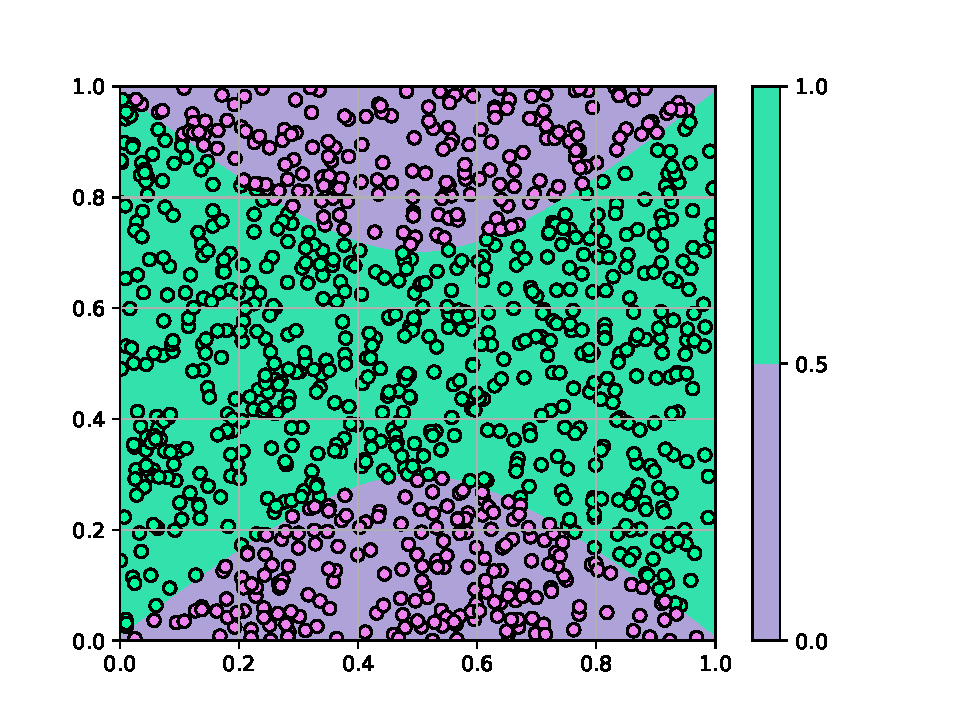
\includegraphics[width=0.75\textwidth]{code/cybenko/classification-example.pdf}
		\caption{Класи $\mathcal{P}_0$ та $\mathcal{P}_1$ на квадраті
		$\mathcal{Q}_2$. Разом з класами, зображено набір данних
		$\mathcal{D}=\{(\mathbf{x}_n,\mathds{1}(\mathbf{x}_n \in
		\mathcal{P}_1))\}_{1 \leq n \leq N} \subset \mathcal{Q}_2 \times
		\{0,1\}$.}
		\label{fig:classification_example}
	\end{figure}

	Питання: якими мають бути параметри для того, щоб функція $\widehat{f}$
	апроксимувала функцію $f$ з гарною точністю? Виявляється, що достатньо
	непоганий результат можна отримати використовуючи наступні параметри:
	\begin{align*}
		\boldsymbol{\alpha} &\approxeq (-8.18, 3.81, 3.91, -3.41, 5.07, 1.16), \\
		\boldsymbol{\beta} &\approxeq (1.13, -2.20, 1.72, 12.47, 8.46, 5.02), \\
		\boldsymbol{W} &\approxeq \begin{bmatrix}
			0.06 & 4.85 & -4.39 & -11.81 & -7.59 & 14.19 \\
			-6.44 & -7.67 & -6.76 & -15.67 & -10.26 & -19.17
		\end{bmatrix}^{\top}.
	\end{align*}
	Помітимо, що ми трошки скоротили запис, сформувавши з параметрів вектори та
	матриці, як це було зроблено у Формулі~\ref{eq:modern_cybenko}.
\end{example}

Зверніть, що на Рис.~\ref{fig:classification_example} ми також зображуємо набір
даних $\mathcal{D}$, що складається з $N=1000$ точок з відповідним маркуванням
(бітом), що відповідає класу, до якого належить точка. Головна причина цього ---
мати спосіб знайти параметри моделі $\widehat{f}$: ми можемо використати, наприклад,
алгоритм градієнтного спуску для мінімізації функції втрат. 

\begin{remark}[Про тренування моделі]
	Забігаючи вперед, для підбору оптимальних параметрів ми використовували
	середньоквадратичну функцію втрати:
	\begin{equation*}
		\mathcal{L}(\mathcal{D}|\boldsymbol{\theta}) = \frac{1}{N}\sum_{n=1}^N \left(\widehat{f}(\mathbf{x}_n|\boldsymbol{\theta}) - y_n\right)^2,
	\end{equation*}
	і далі використовували алгоритм градієнтного спуску (Adam Optimizer \cite{adam}) для мінімізації цього виразу відносно параметрів $\boldsymbol{\theta}$. Більше деталей наведено у Додатку~\ref{appendix:cybenko-code}.
\end{remark}

Після тренування, результати зображені на
Рис.~\ref{fig:classification_result}(а). Помітимо, що вихід
$\widehat{f}(\mathbf{x})$ не є бінарним, але можна ввести поріг $\tau \in
\mathbb{R}$ такий, що передбачення $\widehat{y} := \mathds{1}(\widehat{f}(\mathbf{x}) >
\tau)$ відповідає класу 1 за умови $\widehat{f}(\mathbf{x}) > \tau$, а інакше ---
класу 0. На Рис.~\ref{fig:classification_result}(б) зображено результати
класифікації для $\tau=0.62$. Як бачимо, класифікатор працює досить добре.

\begin{figure}
	\centering
	\begin{subfigure}{0.49\textwidth}
		\centering
		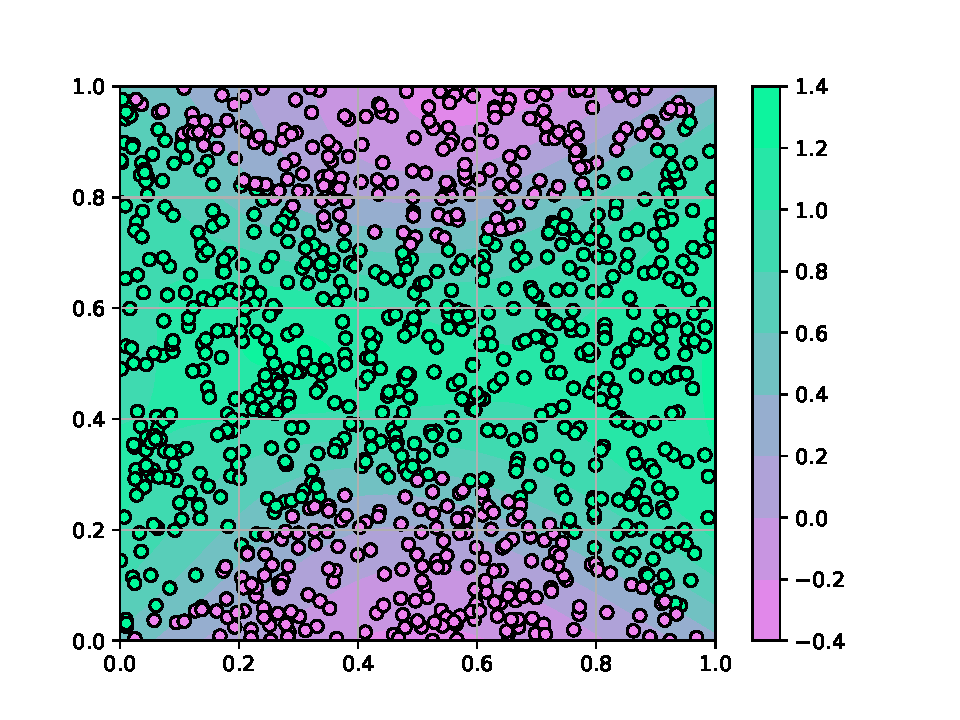
\includegraphics[width=0.99\textwidth]{code/cybenko/classification-cont-prediction.pdf}
		\caption{Результат класифікації $\widehat{f}(\mathbf{x})$ на квадраті $\mathcal{Q}_2$.}
	\end{subfigure}
	\begin{subfigure}{0.49\textwidth}
		\centering
		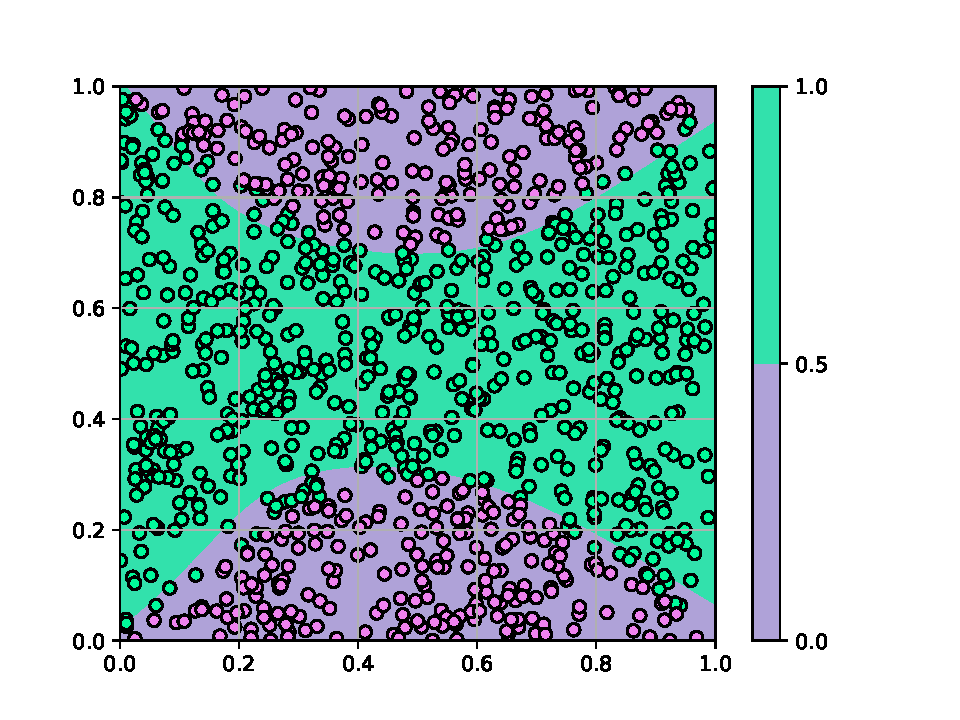
\includegraphics[width=0.99\textwidth]{code/cybenko/classification-discr-prediction.pdf}
		\caption{Бінарний результат класифікації $\mathds{1}(\widehat{f}(\mathbf{x})>\tau)$ з порогом $\tau \approxeq 0.62$.}
	\end{subfigure}
	\caption{Результати класифікації для класів $\mathcal{P}_0$ та $\mathcal{P}_1$ на квадраті $\mathcal{Q}_2$.}
	\label{fig:classification_result}
\end{figure}

Також для цікавості, можна побудувати подібне зображення передбачень, але для 
кожного нейрону. На Рис.~\ref{fig:classification_neuron} зображено результати
передбачень для кожного нейрону у скритому шарі.

\begin{figure}
\begin{tikzpicture}[
    node distance=1.5cm and 1.5cm,
    every node/.style={inner sep=0pt, anchor=center},
    ->, >=Stealth
]
    % Initial image node
    \node (input) {
        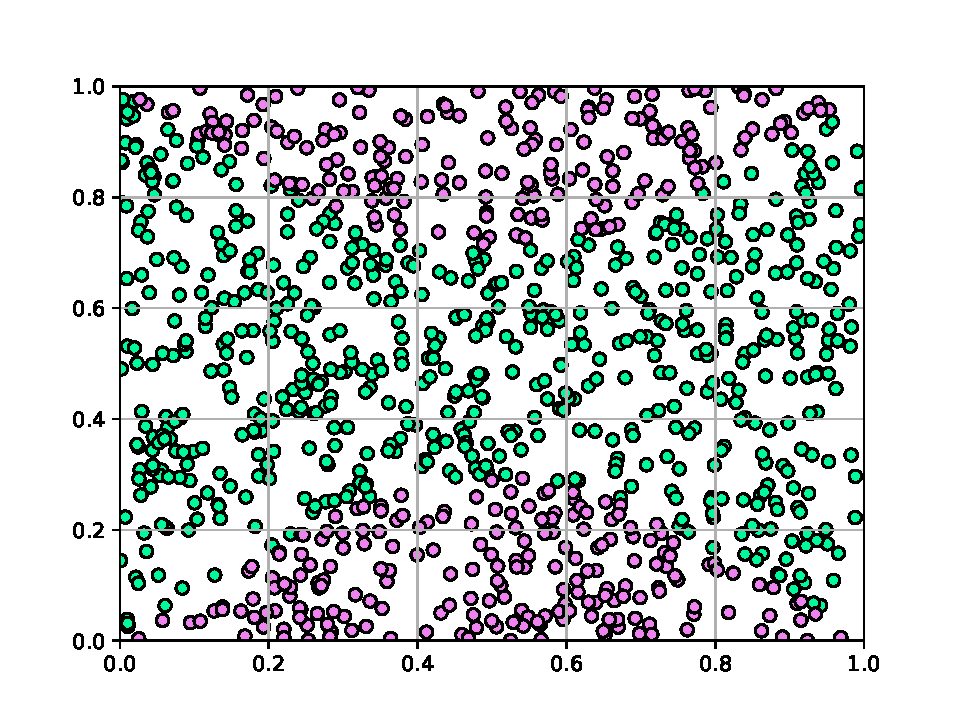
\includegraphics[trim={1cm 0.5cm 3.75cm 1cm},clip,width=6cm]{code/cybenko/dataset.pdf}
    };

    % Hidden layer nodes arranged horizontally below the input
    \foreach \i [count=\j from 1] in {1, 2, 3, 4, 5, 6} {
        \node[below=2.25cm of input, xshift=(\j - 3.5) * 2.75cm] (hidden\i) {
            \includegraphics[trim={1cm 0.5cm 3.75cm 1cm},clip,width=2.75cm]{code/cybenko/layer-\i-prediction.pdf}
        };
        % Connect input to each hidden layer node
        \draw[ultra thick,-{Stealth[length=3.5mm]}] (input.south) -- (hidden\i.north);
    }

    % Final prediction node centered below the hidden layer
    \node[yshift=-12.5cm, xshift=-4.0cm] (output) {
        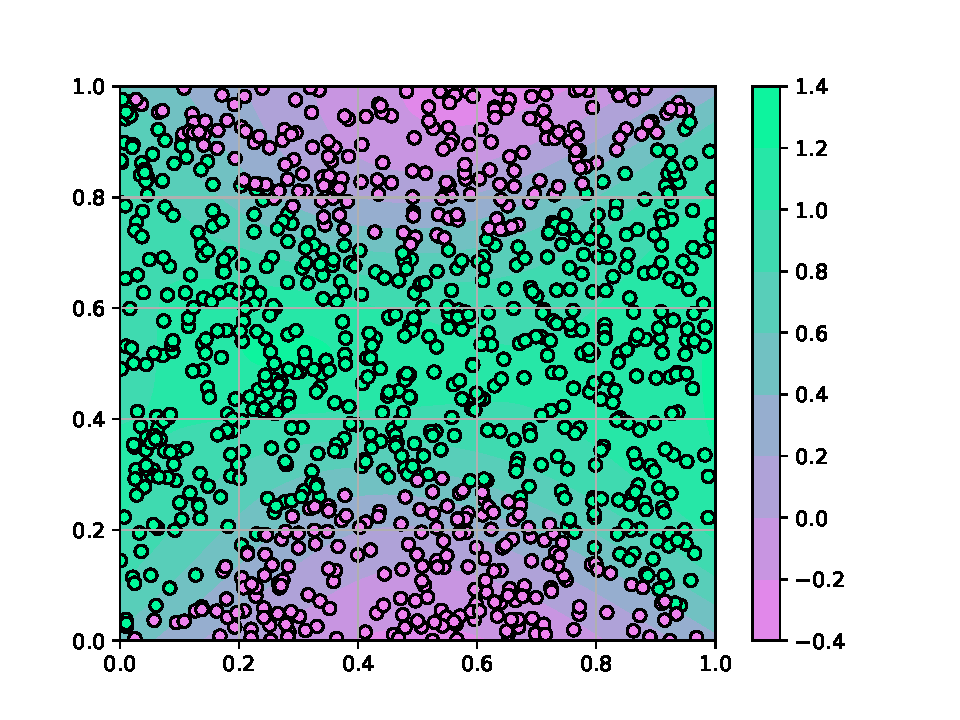
\includegraphics[trim={1cm 0.5cm 3.75cm 1cm},clip,width=6cm]{code/cybenko/classification-cont-prediction.pdf}
    };

	% Discrete prediction node right to the final prediction
	\node[right=2.5cm of output] (discrete) {
		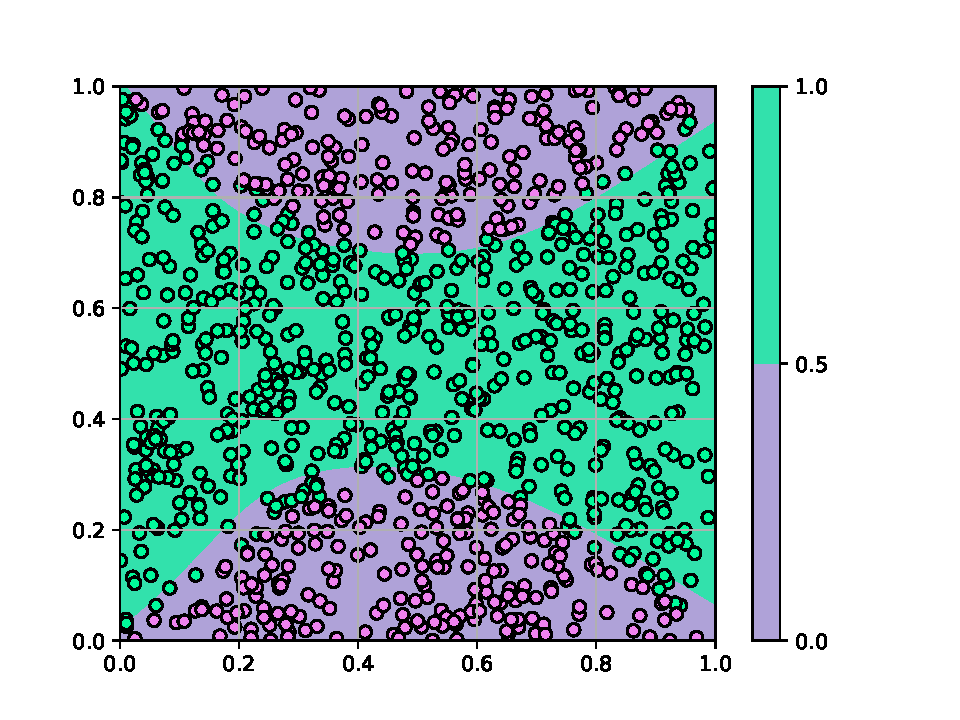
\includegraphics[trim={1cm 0.5cm 3.75cm 1cm},clip,width=6cm]{code/cybenko/classification-discr-prediction.pdf}
	};

    % Connect hidden layer nodes to final output
    \foreach \i in {1, 2, 3, 4, 5, 6} {
        \draw[ultra thick,-{Stealth[length=3.5mm]}] (hidden\i.south) -- (output.north);
    }

	% Draw a transparent green rectangle line on the level of the input layer and 
	% make a transparent green background for the input layer
	\scoped[on background layer]\draw[green!50!black, fill=green, line width=0.5mm,
	fill opacity=0.2,dashed] ([xshift=-2.5cm,yshift=0.5cm]input.north west) rectangle ([xshift=2.5cm,yshift=-0.5cm]input.south east);

	% Same for hidden layer with a blue color and orange for output
	\scoped[on background layer]\draw[blue!50!black, fill=blue, line width=0.5mm,
	fill opacity=0.2,dashed] ([xshift=-8.5cm,yshift=0.5cm]hidden3.north east) rectangle ([xshift=8.5cm,yshift=-0.5cm]hidden3.south east);
	\scoped[on background layer]\draw[orange!50!black, fill=orange, line width=0.5mm,
	fill opacity=0.2,dashed] ([xshift=-6.5cm,yshift=0.10cm]output.north east) rectangle ([xshift=9.0cm,yshift=-0.10cm]output.south east);

	% Labels written verfically left to the boxes
	\node[rotate=90] at ([xshift=-6.0cm]input) {\textcolor{green!80!black}{\textbf{Вхідний шар}}};
	\node[rotate=90] at ([xshift=-7.50cm]hidden3) {\textcolor{blue!80!black}{\textbf{Скритий шар}}};
	\node[rotate=90] at ([xshift=-4.0cm]output) {\textcolor{orange!80!black}{\textbf{Вихідний шар}}};

	% Between input layer and hidden layer, write down x -> w^T x + b in a box with fill
	\node[below=0.60cm of input, fill=blue!20!white, dashed, minimum size=1cm, text width=5cm, align=center, rounded corners=.55cm] {\normalsize$\mathbf{x} \xrightarrow{\boldsymbol{w}^{\top}_j\mathbf{x} + \beta_j} \Sigma_j \xrightarrow{\sigma} z_j$};

	% Between hidden layer and output layer, write down sum of z_j * alpha_j
	\node[above=0.40cm of output, fill=orange!20!white, dashed, minimum size=1cm, text width=5cm, align=center, rounded corners=.55cm] {\normalsize$\widehat{f}(\mathbf{x}) \gets \langle \boldsymbol{\alpha}, \mathbf{z} \rangle$};

	% And arrow as well with a text
	\draw[ultra thick,-{Stealth[length=3.5mm]}] (output.east) -- (discrete.west) node[midway, above=0.25cm, align=center] {Поріг $\tau$};
\end{tikzpicture}

\caption{Результати передбачень для кожного нейрону у скритому шарі.}
\label{fig:classification_neuron}

\end{figure}

\subsection{Подальший розвиток архітектури Цибенко}

Звичайно, що науковці не зупинились на результатах Цибенко. В подальших 
архітектурах, дослідники ставили багато питань, таких як:
\begin{itemize}
	\item Що, якщо зробити кілька скритих шарів у мережі?
	\item Чи можна використовувати інші активаційні функції окрім сігмоїдів?
	\item А чи можна поєднувати два скритих шара іншим способом?
\end{itemize}

Саме тому, була введена багатошарова модель персептронів (Multi-Layer
Perceptrons --- MLP), яку ми сформулюємо нижче.
\begin{definition}[Багатошарова модель персептронів]\label{def:mlp}
	Нехай $\ell \in \mathbb{N}$ --- кількість шарів у мережі, а
	$n_0,\dots,n_{\ell} \in \mathbb{N}$ --- кількість нейронів у кожному шарі,
	де $\mathbf{x}^{\langle 0 \rangle} \in \mathbb{R}^{n_0}$ відповідає вхідному
	шару. Тоді, для знаходження виходу $\mathbf{x}^{\langle \ell \rangle} \in
	\mathbb{R}^{n_{\ell}}$, багатошарова модель персептронів використовує
	наступне рекурентне правило:
	\begin{equation*}
		\mathbf{x}^{\langle j+1 \rangle} = \phi^{\langle j \rangle}(\mathbf{z}^{\langle j \rangle}), \quad \mathbf{z}^{\langle j \rangle} = \boldsymbol{W}^{\langle j \rangle}\mathbf{x}^{\langle j \rangle} + \boldsymbol{\beta}^{\langle j \rangle}, \quad j = 0,\dots,\ell-1,
	\end{equation*}
	де $\phi^{\langle j \rangle}$ --- активаційна функція у шарі $j$, а
	$\boldsymbol{W}^{\langle j \rangle} \in \mathbb{R}^{n_{j+1} \times n_j}$ та
	$\boldsymbol{\beta}^{\langle j \rangle} \in \mathbb{R}^{n_{j+1}}$ ---
	матриця ваг та вектор зсуву у шарі $j$ відповідно. Таким чином,
	параметризація моделі є $\boldsymbol{\theta} =
	\left\{\boldsymbol{W}^{\langle j \rangle},\boldsymbol{\beta}^{\langle j
	\rangle}\right\}_{0 \leq j \leq \ell-1}$.
\end{definition}

\subsubsection{Навіщо більше шарів?}

Здавалося б, якщо ми можемо апроксимувати будь-яку функцію за допомогою одного
скритого шару, то навіщо нам багатошарові моделі? Виявляється, що більше шарів
дозволяють нам апроксимувати складніші функції за допомогою меншої кількості
нейронів і чисельно знаходити їх стає простіше. Емпірично, набір правил, що
описують ефективність моделі від кількості тренувальних параметрів, розміру
набору даних та інших факторів, називають законами масштабування
(\textit{Scaling Laws}). Зокрема, емпірично, середнє значення функції втрати $L$
залежить від кількості параметрів $N$ як $L \propto N^{-\alpha}$ для певної
константи $\alpha>0$. Більш детальне дослідження від інших параметрів таких як
гіперпараметри архітектури, розміру набору даних можна подивитися у джерелі
\cite{scaling}. Зокрема, джерело \cite{params-generalization} строго показує
асимптотичну залежність між кількістю параметрів та загальнізацією моделі для
задачі класифікації, а джерело \cite{params-generalization-2} доводить, що якщо
розмір вибірки $D$ і вхід складається з $m$ нейронів, то при кількості
параметрів $N=(D/(m\log D))^{1/2}$, то, асимтотично, $L_2$ норма різниці між
апроксимацією та реальною функцією обмежена як $\mathcal{O}((m/D)\log D)^{1/2}$.

\subsubsection{Навіщо інші активаційні функції?}
Окрім того, на практиці, логістична функція виявляється дуже незручною. Зокрема,
вона відноситься до класу функцій, що називаються \textit{ненасиченими} (або
\textit{non-saturating activation function}). Основна проблема полягає у тому,
що під час навчання моделі, ми використовуємо градієнтні методи, які полагаються
на значення матриці Якобіана функції втрати відносно параметрів моделі.
Спрощено, моделі змінюються на мале значення $\delta\boldsymbol{\theta}
\approxeq \eta
(\partial\mathcal{L}/\partial\boldsymbol{\theta})\Big|_{\boldsymbol{\theta}=\boldsymbol{\theta}_{\text{current}}}$.
У ході обчислення цього градієнту, ми використовуємо правило ланцюга, що
призводить до того, що кожен доданок у виразі містить вираз $\sigma'(z)$ у
добутку. Для логістичної функції, похідна $\sigma'(z) = \sigma(z)(1-\sigma(z))$ і
легко бачити, що як для малих, так і для великих значень $z$, ця похідна
дуже стрімко наближається до нуля, що призводить до проблеми \textit{вицідження
градієнту} (\textit{vanishing gradient problem}). Це означає, що градієнт
функції втрати може бути дуже малим, що призводить до того, що модель не
навчається. Зокрема, нижче ми наводимо популярні функції, що використовують 
для розв'язку цієї проблеми:
\begin{enumerate}
	\item \textbf{ReLU} (Rectified Linear Unit): $\phi(z) = \max\{0,z\}$. Ця 
	функція має похідну $\phi'(z) = \mathds{1}(z>0)$, тобто за додатніх
	значень $z$ градієнт не виціджується. Проте, для від'ємних значень $z$,
	градієнт нульовий, через що модель може ``тормозити''. Для виріження цієї 
	проблеми, було запропоновано модифікації ReLU, такі як Leaky ReLU.
	\item \textbf{Leaky ReLU}: $\phi(z) = \max\{\alpha z,z\}$ де $\alpha \in
	[0,1)$ --- мале значення (на практиці, порядку $10^{-3}$). Ця функція має
	похідну $\phi'(z)\Big|_{z<0} = \alpha$, що дозволяє градієнту не
	виціджуватись для від'ємних значень $z$.
	\item \textbf{ELU} (Exponential Linear Unit): $\phi(z) =
	\max\{0,z\}+\min\{\alpha(e^z-1),0\}$, де $\alpha$ --- додатне значення. Ця
	функція має похідну $\phi'(z)\Big|_{z<0} = \alpha e^z$. За великих від'ємних
	значень $z$, ця функція збігається з ReLU, але має неперервну та нестрого
	нульову похідну для від'ємних значень $z$.
\end{enumerate}

\subsubsection{Інша архітектура}

Ще одним питанням, яке виникає, це як поєднувати шари у мережі. Поки що, логіка
така: кожен нейрон $i$ у шарі $\ell$ з'єднаний з кожним нейроном $j$ у шарі
$\ell+1$ з певною вагою $w_{i,j}^{\langle \ell \rangle}$ (що і утворюють матрицю
ваг $\boldsymbol{W}^{\langle \ell \rangle}$). Проте, чи дійсно нам потрібно 
стільки зв'язків? І чи дійсно така репрезентація здатна відобразити достатньо
складні стосунки за малу кількість параметрів? Виявляється, що для певних задач
можна використовувати інші архітектури. Нижче наведемо два приклади, що 
показують проблематику зв'язків у мережі.

\begin{example}
	Уявіть, що вам потрібно побудувати бінарну класифікацію для кольорового
	зображення відносно невеликого розміру --- скажімо, $200 \times 200$
	пікселів. Якщо у якості входу взяти кожен окремий піксель як нейрон, то
	кількість параметрів у першому шарі буде $200 \times 200 \times 3 = 120000$.
	Уявімо, що у скритий шар ми поставимо буквально 10 нейронів (на практиці,
	така кількість мала для досягнення хорошої точності). Таким чином, кількість
	параметрів у моделі буде як мінімум $120000 \times 10 = 1.2$ млн. 
\end{example}

\begin{example}
	Що робити, якщо розмір входу та виходу, взагалі кажучи, не фіксовані 
	(наприклад, обробка тексту)? Звичайно, можна задати ``зазделегідь''
	максимальний розмір входу та виходу, але окрім аномальної кількості
	параметрів, точність такої моделі може бути дуже низькою.
\end{example}

У рамках цієї курсової роботи, ми не беремось за повний і строгий опис всіх
сучасних архітектур, проте навели основний фундамент для подальшого вивчення
глибокого навчання. Для більш детального огляду, рекомендуємо звернутися до
джерел \cite{book-1,book-2}.

\section{Теорема Колмогорова-Арнольда}

\subsection{Історія та Мотивація}

Ще один дуже цікавий спосіб підходу до апроксимації функцій --- це використання
теореми Колмогорова-Арнольда. Історично, ця теорема походить з 13 задачі
Гільберта, яка була запропонована на Паризькому конгресі математиків у 1900 році.
Вона задає доволі провокативне питання: а чи існують справді неперервні 
дійснозначні багатовимірні функції? Здавалося б, доволі дивне запитання,
але воно по суті і описує 13 задачу і, відповідно, її розв'язок --- теорему
Колмогорова-Арнольда. 

Більш конкретно, питання полягає у тому, чи можна будь-яку, скажімо, неперервну
функцію $f: \mathcal{Q}_m \to \mathbb{R}$ апроксимувати за допомогою суми та
композицій певного набору одновимірних неперервних функцій
$\phi_1,\dots,\phi_N$? Розглянемо декілька прикладів на основі
\cite{ka-explained}, щоб показати суть цієї задачі.

\begin{example}
	Нехай $f: \mathcal{Q}_2 \to \mathbb{R}$ задана як $f(x,y) = 3x+5y$. Якщо
	позначити $\phi_1(x)=3x$, $\phi_2=5y$, то $f(x,y) = \phi_1(x)+\phi_2(y)$.
	Отже, маємо функцію двох змінних, проте вона може бути записана як сума двох
	функцій однієї змінної.
\end{example}

\begin{example}
	Попередній приклад здається зовсім тривіальним. А що, якщо $f(x,y)=xy$? Помітимо 
	наступне\footnote{Тут і далі під записом $\log$ розуміємо натуральний логарифм}:
	\begin{equation*}
		f(x,y) = xy = e^{\log (x+1) + \log(y+1)} + \left(-x-0.5\right) + \left(-y-0.5\right).
	\end{equation*}
	Нехай $\phi_1(x) := e^x$, $\phi_2(x) := \log(x+1)$,
	$\phi_3 := -x-0.5$. Тоді:
	\begin{equation*}
		f(x,y) = \phi_1(\phi_2(x)+\phi_2(y)) + \phi_3(x) + \phi_3(y).
	\end{equation*}

	Отже, функція $f(x,y)$ може бути записана як сума та композиція функцій
	однієї змінної $\phi_1(x),\phi_2(x),\phi_3(x)$.
\end{example}

\begin{example}
	Нехай $f(x,y) = \sin (10e^x + y^{100})$, а також $\phi_1(x) := 10e^x,
	\phi_2(x) := y^{100}$ та $\phi_3(x) := \sin x$. Тоді $f(x,y) =
	\phi_3(\phi_1(x)+\phi_2(y))$, тобто так само маємо $f(x,y)$ як композицію та
	суму одновимірних функцій.
\end{example}

Отже, на основі цих прикладів можна зрозуміти суть 13 проблеми Гільберта.
\begin{statement}[Основна гіпотеза 13 проблеми Гільберта]
	Існує неперервна функція $f: \mathcal{Q}_3 \to \mathbb{R}$, що не може бути
	виражена як композиція та сума неперервних функцій $\phi_1,\dots,\phi_N \in
	\mathcal{C}(\mathbb{R}^2)$.
\end{statement}

Знадобилося більше 50 років для того, щоб довести, що це твердження
\textit{хибне}. У 1956 році Колмогоров довів, що функція будь-якої кількості
змінних (себто, $\mathcal{Q}_m$ може бути довільним гіперкубом) може бути
записана як сума та композиція трьохвимірних функцій. У 1957, у 19 років,
Арнольд показав, що три змінні можна замінити на дві, що власне і розв'язує в
більш загальному вигляді 13 проблему Гільберта. Нарешті, згодом Колмогоров 
показав, що дві змінні можна замінити на одну, що врешті-решт і дає 
відому теорему Колмогорова-Арнольда.

\begin{theorem}[Згідно джерелу \cite{ka-explained}]
	Для будь-якого натурального $m \geq 2$, існують неперервні функції
	$\phi_1,\dots,\phi_{2m+1} \in \mathcal{C}([0,1])$ та дійсні числа
	$\lambda_1,\dots,\lambda_m \in \mathbb{R}$ з такою властивістю, що для
	будь-якої функції $f \in \mathcal{C}(\mathcal{Q}_m)$ знайдеться неперервна
	функція $\Phi: \mathbb{R} \to \mathbb{R}$ така, що для будь-якого
	$\mathbf{x} = (x_1,\dots,x_m) \in \mathcal{Q}_m$ справедливо:
	\begin{equation*}
		f(\mathbf{x}) = \sum_{q=1}^{2m+1}\Phi\left(\sum_{p=1}^{m}\lambda_p\phi_q(x_p)\right)
	\end{equation*}
\end{theorem}

\begin{remark}\label{remark:ka-remark}
	В цій формулі дуже багато чого цікавого! По-перше, дивує сам факт не наближеної
	апроксимації, а точної рівності. По-друге, важливо помітити, що функції
	$\phi_1,\dots,\phi_{2m+1}$ не залежать від $f$, але залежать від $m$. Це
	означає, що ми можемо знайти ці функції один раз, і вони будуть працювати для
	будь-якої функції $f$! Після чого залишиться лише знайти $\Phi$.
\end{remark}

Здавалося б, враховуючи Зауваження~\ref{remark:ka-remark}, чому ми не можемо
спочатку знайти ці функції, а потім використовувати їх у прикладних задачах?
Річ у тому, що ніхто не гарантує, що ці функції взагалі мають бути диференційованими
і тим паче неперервно диференційованими. Саме тому, подальший пошук функції $\Phi$
автоматично стає майже неможливим завданням. Тому, як ми можемо використовувати
теорему Колмогорова-Арнольда для побудови нейронних мереж?

\subsection{Мережі Колмогорова-Арнольда}

Довгий час ідею теореми Колмогорова-Арнольда не пробували застосовувати до
глибокого навчання через ``поганість'' функцій $\Phi,\phi_1,\dots,\phi_{2m+1}$.
Проте, буквально у цьому році найпоширенішою темою дискусії у суспільстві
розробників глибокого навчання стала робота ``KAN: Kolmogorov-Arnold Networks''
\cite{kan}. По суті, до моменту публікації, єдина парадигма апроксимації функцій
полягала у побудові MLP мереж (та їх подальших варіацій у вигляді конволюційних,
рекурентних мереж тощо), що грунтується на вище описаній універсальній теоремі
апроксимації \ref{theorem:cybenko_1}. Однак, автори роботи \cite{kan} показали,
що і на основі репрезентації Колмогорова-Арнольда можна побудувати нейронні мережі. 
Яким чином?

Робота \cite{kan} використовує оригінальну теорему Колмогорова-Арнольда \cite{kolmogorov-original}.
\begin{definition}[Оригінальна теорема Колмогорова \cite{kolmogorov-original}]
	Для будь-якого натурального $m \geq 2$, існують неперервні функції
	$\phi_{p,q} \in \mathcal{C}([0,1])$ такі, що для будь-якої функції $f \in
	\mathcal{C}(\mathcal{Q}_m)$ знайдуться неперервні функції
	$\Phi_1,\dots,\Phi_{2m+1} \in \mathcal{C}(\mathbb{R})$ такі, що
	\begin{equation*}
		f(x_1,\dots,x_m) = \sum_{q=1}^{2m+1}\Phi_q\left(\sum_{p=1}^n \phi_{p,q}(x_p)\right)
	\end{equation*}
\end{definition}

Проте, як і для Означення~\ref{def:mlp} MLP мереж, нам потрібно вміти узагальнювати
означення для довільної кількості шарів та нейронів в кожному шарі. Робота 
\cite{kan} стала першою, що запропонувала таку узагальнену модель. Спочатку,
наведемо що є \textit{з'єднанням в KAN мережі}.

\begin{definition}
	\textbf{З'єднання KAN Мережі} між шаром з $n_{\text{in}} \in \mathbb{N}$
	нейронами (активаціями) та шаром з $n_{\text{out}} \in \mathbb{N}$ нейронами
	складається з матриці функцій $\boldsymbol{\Phi} = \{\phi_{q,p}\}_{1\leq
	p\leq n_{\text{in}}, 1 \leq q \leq n_{\text{out}}}$, де кожна функція
	$\phi_{q,p}: \mathbb{R} \to \mathbb{R}$ параметризується параметрами
	$\boldsymbol{\theta}_{q,p}$. Значення нейронів (активацій)
	$\mathbf{x}_{\text{out}} \in \mathbb{R}^{n_{\text{out}}}$ через попередні
	нейрони $\mathbf{x}_{\text{in}} \in \mathbb{R}^{n_{\text{in}}}$ визначається
	згідно рівнянню $\mathbf{x}_{\text{out}} = \boldsymbol{\Phi} \circ
	\mathbf{x}_{\text{in}}$, де під виразом $\boldsymbol{\Phi} \circ
	\mathbf{x}_{\text{in}} \in \mathbb{R}^{n_{\text{out}}}$, по аналогії з
	матричним добутком, мається на увазі:
	\begin{equation*}
		(\boldsymbol{\Phi} \circ \mathbf{x}_{\text{in}})_j = \sum_{i=1}^{n_{\text{in}}}\phi_{j,i}(x_{\text{in},i}), \quad j \in \{1,\dots,n_{\text{out}}\}.
	\end{equation*}
\end{definition}

Отже, ми можемо дати означення безпосередньо мережі.
\begin{definition}[Архітектура KAN]
	Нехай $\ell \in \mathbb{N}$ --- кількість шарів у мережі, а
	$n_0,\dots,n_{\ell} \in \mathbb{N}$ --- кількість нейронів у кожному шарі,
	де $\mathbf{x}^{\langle 0 \rangle} \in \mathbb{R}^{n_0}$ відповідає вхідному
	шару. Тоді, для знаходження виходу $\mathbf{x}^{\langle \ell \rangle} \in
	\mathbb{R}^{n_{\ell}}$, архітектура KAN використовує рекурентне правило
	$\mathbf{x}^{\langle j+1 \rangle} = \boldsymbol{\Phi}^{\langle j \rangle}
	\circ \mathbf{x}^{\langle j \rangle}$, $j \in \{0,\dots,\ell-1\}$, де
	$\boldsymbol{\Phi}^{\langle j \rangle} =
	\{\phi^{\langle j \rangle}_{q,p}\}_{1\leq p\leq n_j, 1 \leq q \leq
	n_{j+1}}$ --- матриця функцій-ваг $j$. В розгорнутому вигляді, нейронна мережа $\widehat{f}_{\text{KAN}}$ записується як:
	\begin{equation*}
		\widehat{f}_{\text{KAN}}(\mathbf{x}) = \left(\bigcirc_{j=1}^{\ell}\boldsymbol{\Phi}^{\langle \ell - j \rangle}\right)\circ \mathbf{x}
	\end{equation*}
\end{definition}

Таке визначення може здатися доволі заплутаним, тому давайте розглянемо приклад.

\begin{example}[Теорема Арнольда як частковий випадок KAN]
	Нагадаємо, що теорема Колмогорова-Арнольда стверджує, що будь-яка функція 
	$f \in \mathcal{C}(\mathcal{Q}_m)$ може бути записана як
	\begin{equation*}
		f(x_1,\dots,x_m) = \sum_{q=1}^{2m+1}\Phi_q\left(\sum_{p=1}^m \phi_{p,q}(x_p)\right).
	\end{equation*}

	Тоді, якщо ми визначимо дві матриці-ваги $\boldsymbol{\Phi}^{\langle 0 \rangle} = \{\phi_{p,q}\}_{1 \leq p \leq m, 1 \leq q \leq 2m+1}$ та
	$\boldsymbol{\Phi}^{\langle 1 \rangle} = \{\Phi_q\}_{1 \leq q \leq 2m+1}$ (матриця-рядок), то ми можемо записати
	\begin{equation*}
		f(x_1,\dots,x_m) = \widehat{f}_{\text{KAN}}(x_1,\dots,x_m) = \boldsymbol{\Phi}^{\langle 1 \rangle} \circ \boldsymbol{\Phi}^{\langle 0 \rangle} \circ \mathbf{x}
	\end{equation*}
\end{example}

Отже, залишається лише обрати параметризацію для кожної функції
$\phi_{p,q}^{\langle j \rangle}$. Оригінальна робота \cite{kan} пропонує 
використовувати лінійну комбінацію певної фіксованої базисної функції $\beta(x)$ та $B$-сплайн порядку $d$:
\begin{equation*}
	\phi_{p,q}^{\langle j \rangle}(x) = \omega_{\beta} \beta(x) + \omega_S\sum_{k=1}^{d} \theta_{p,q,k}^{\langle j \rangle} B_{k,d}(x),
\end{equation*}
де $B_{k,d}(x)$ --- $k$-тий $B$-сплайн порядку $d$, $\theta_{p,q,k}^{\langle j
\rangle}$ --- параметри моделі і $\omega_{\beta},\omega_S$ --- фіксовані ваги
для базисної функції та $B$-сплайнів відповідно (що є гіперпараметрами). В
роботі пропонується обрати $\beta(x) := x\sigma(x)$. 

Архітектура KAN для двох шарів зображена на Рис.~\ref{fig:kan-architecture}.

\begin{figure}
\centering
\begin{tikzpicture}[node distance=1.5cm, every node/.style={align=center}]
    % Layer 0 (Input Layer)
    \node[circle, draw, ultra thick, green!50!black, fill=green!20, minimum size=0.5cm] (x01) {$x_{1}^{\langle 0 \rangle}$};
    \node[circle, draw, ultra thick, green!50!black, fill=green!20, minimum size=0.5cm, right=1cm of x01] (x02) {$x_{2}^{\langle 0 \rangle}$};

    % Applying phi functions
    \node[rectangle, draw, ultra thick, blue!50!black, fill=blue!20, minimum width=1cm, minimum height=1cm, above left=1.5cm and 3.0cm of x01, rounded corners=.20cm] (phi11) {$\phi_{1,1}^{\langle 0 \rangle}$};
    \node[rectangle, draw, ultra thick, blue!50!black, fill=blue!20, minimum width=1cm, minimum height=1cm, above left=1.5cm and 1.5cm of x01, rounded corners=.20cm] (phi21) {$\phi_{2,1}^{\langle 0 \rangle}$};
    \node[rectangle, draw, ultra thick, blue!50!black, fill=blue!20, minimum width=1cm, minimum height=1cm, above left=1.5cm and 0.0cm of x01, rounded corners=.20cm] (phi31) {$\phi_{3,1}^{\langle 0 \rangle}$};
    
	\node[rectangle, draw, ultra thick, blue!50!black, fill=blue!20, minimum width=1cm, minimum height=1cm, above right=1.5cm and 0.0cm of x02, rounded corners=.20cm] (phi12) {$\phi_{1,2}^{\langle 0 \rangle}$};
    \node[rectangle, draw, ultra thick, blue!50!black, fill=blue!20, minimum width=1cm, minimum height=1cm, above right=1.5cm and 1.5cm of x02, rounded corners=.20cm] (phi22) {$\phi_{2,2}^{\langle 0 \rangle}$};
    \node[rectangle, draw, ultra thick, blue!50!black, fill=blue!20, minimum width=1cm, minimum height=1cm, above right=1.5cm and 3.0cm of x02, rounded corners=.20cm] (phi32) {$\phi_{3,2}^{\langle 0 \rangle}$};
    
    % Finding new activations (Layer 1)
    \node[circle, draw, ultra thick, gray!80!black, fill=gray!20, minimum size=1cm, above right=5.0cm and 0.5cm of x01] (x12) {$\boldsymbol{\Sigma}$};
    \node[circle, draw, ultra thick, gray!80!black, fill=gray!20, minimum size=1cm, left=1.5cm of x12] (x11) {$\boldsymbol{\Sigma}$};
    \node[circle, draw, ultra thick, gray!80!black, fill=gray!20, minimum size=1cm, right=1.5cm of x12] (x13) {$\boldsymbol{\Sigma}$};

	% Draw labels left to each sum node
	\node[left=-0.15cm of x11, font=\small, gray!80!black] {$x_1^{\langle 1 \rangle}$};
	\node[left=-0.15cm of x12, font=\small, gray!80!black] {$x_2^{\langle 1 \rangle}$};
	\node[left=-0.15cm of x13, font=\small, gray!80!black] {$x_3^{\langle 1 \rangle}$};

	% Drawing phi functions above Layer 1
	\node[rectangle, draw, ultra thick, blue!50!black, fill=blue!20, minimum width=1cm, minimum height=1cm, above=1cm of x11, rounded corners=.20cm] (phi111) {$\phi_{1,1}^{\langle 1 \rangle}$};
	\node[rectangle, draw, ultra thick, blue!50!black, fill=blue!20, minimum width=1cm, minimum height=1cm, above=1cm of x12, rounded corners=.20cm] (phi121) {$\phi_{1,2}^{\langle 1 \rangle}$};
	\node[rectangle, draw, ultra thick, blue!50!black, fill=blue!20, minimum width=1cm, minimum height=1cm, above=1cm of x13, rounded corners=.20cm] (phi131) {$\phi_{1,3}^{\langle 1 \rangle}$};

	% Layer 3: Draw orange output above x12 at distance 1cm
	\node[circle, draw, ultra thick, orange!80!black, fill=orange!20, minimum size=1cm, above=1.0cm of phi121] (x21) {$x_{1}^{\langle 2 \rangle}$};

    % Connections between layers
    \draw[ultra thick,-{Stealth[length=3.5mm]}] (x01) -- (phi11);
	\draw[ultra thick,-{Stealth[length=3.5mm]}] (x01) -- (phi21);
	\draw[ultra thick,-{Stealth[length=3.5mm]}] (x01) -- (phi31);

	\draw[ultra thick,-{Stealth[length=3.5mm]}] (x02) -- (phi12);
	\draw[ultra thick,-{Stealth[length=3.5mm]}] (x02) -- (phi22);
	\draw[ultra thick,-{Stealth[length=3.5mm]}] (x02) -- (phi32);
	
	% Connect the phi functions to the sum nodes
	\draw[ultra thick,-{Stealth[length=3.5mm]}] (phi11) -- (x11);
	\draw[ultra thick,-{Stealth[length=3.5mm]}] (phi12) -- (x11);
	\draw[ultra thick,-{Stealth[length=3.5mm]}] (phi21) -- (x12);
	\draw[ultra thick,-{Stealth[length=3.5mm]}] (phi22) -- (x12);
	\draw[ultra thick,-{Stealth[length=3.5mm]}] (phi31) -- (x13);
	\draw[ultra thick,-{Stealth[length=3.5mm]}] (phi32) -- (x13);

	% Connect the sum nodes to the phi functions in Layer 1
	\draw[ultra thick,-{Stealth[length=3.5mm]}] (x11) -- (phi111);
	\draw[ultra thick,-{Stealth[length=3.5mm]}] (x12) -- (phi121);
	\draw[ultra thick,-{Stealth[length=3.5mm]}] (x13) -- (phi131);

	% Connect the phi functions in Layer 1 to the output node
	\draw[ultra thick,-{Stealth[length=3.5mm]}] (phi111) -- (x21);
	\draw[ultra thick,-{Stealth[length=3.5mm]}] (phi121) -- (x21);
	\draw[ultra thick,-{Stealth[length=3.5mm]}] (phi131) -- (x21);

    % Annotations
    \node[right=0.5cm of x02, green!50!black] {\textbf{Input Layer}};
    \node[right=0.5cm of x13, gray!80!black] {\textbf{Hidden Layer}};
    \node[right=0.5cm of x21, orange!80!black] {\textbf{Output Layer}};
\end{tikzpicture}
\caption{Приклад KAN архітектури з трьома шарами з кількістю нейронів $n_0=2$, $n_1=3$, $n_2=1$.}
\label{fig:kan-architecture}
\end{figure}

Єдине, що ми ще не врахували --- а чому така репрезентація взагалі дає універсальну 
апроксимацію на компакті $\mathcal{Q}_m$? Дійсно, хоч теорема Колмогорова-Арнольда
дає точну рівність, але ми поки ніяк не гарантуємо, що якщо замінити функції 
$\{\phi_{p,q}\}$ на $B$-сплайни, то ми все одно можемо апроксимувати будь-яку
функцію. Це питання досліджується в роботі \cite{kan}, де показана наступна теорема.

\begin{theorem}[Теорема апроксимації KAN]
	Нехай функція $f$ має вигляд $f = \boldsymbol{\Phi}^{\langle\ell\rangle}
	\circ \dots \circ \boldsymbol{\Phi}^{\langle 0\rangle} \circ \mathbf{x}$, де
	усі функції $\phi_{p,q}^{\langle j \rangle}$ є $d+1$ разів неперервно
	диференційовані. Тоді, існує така константа $\gamma$, що залежить від $f$ і
	функцій $\{\phi_{p,q}\}$, та існують матриці
	$\widetilde{\boldsymbol{\Phi}}^{\langle\ell\rangle},\dots,\widetilde{\boldsymbol{\Phi}}^{\langle
	0\rangle}$, що складаються з $B$-сплайнів порядку $d$ і розміром сітки $n_G$, що
	для всіх $0 \leq r \leq d$ маємо
	\begin{equation*}
		\left\| f - \widetilde{\boldsymbol{\Phi}}^{\langle\ell\rangle}
		\circ \dots \circ \widetilde{\boldsymbol{\Phi}}^{\langle 0\rangle} \circ \mathbf{x} \right\|_{C^r} \leq \gamma n_G^{r-(d+1)},
	\end{equation*}
	де $\|g\|_{C^r} = \sup_{|\beta|\leq r}\sup_{\mathbf{x} \in \mathcal{Q}_m}|g^{(\beta)}(\mathbf{x})|$.
\end{theorem}

\subsection{Порівняння з MLP архітектурою}

Отже, що краще: MLP чи KAN? Наведемо деякі переваги та недоліки кожної з архітектур.

\begin{enumerate}
	\item \textbf{Кількість інструментів.} Оскільки останні 10 років було
	присвячено розвитку MLP архітектур, то для них існує набагато більше
	інструментів, бібліотек та фреймворків. Навіть якщо KAN має потенціал, то
	простий налаштунок та тренування може стати викликом.
	\item \textbf{Інтерпретованість.} Оскільки KAN використовує $B$-сплайни, то
	вони є більш інтерпретованими, ніж MLP. Це може бути корисним для задач, де
	важливо зрозуміти, як саме мережа приймає рішення.
	\item \textbf{Швидкість тренування.} Згідно з роботою \cite{kan}, KAN мережі
	поки приблизно в $10\times$ повільніші за MLP під час тренування. Проте,
	на практиці, цей показник часто не є критичним: значно більш важливою є
	точність та швидкість обчислення під час обрахунку передбачення.
	\item \textbf{Швидкість передбачення.} Для простоти аналізу, нехай маємо дві
	мережі, написані як на MLP, так і на KAN, у якої $\ell$ шарів, в кожному з
	яких $n$ нейронів і активаційна функція має степінь $d$. Тоді, кількість
	операцій для MLP мережі буде $\mathcal{O}(\ell n(n+d))$: на кожному переході
	між шарами, маємо $n^2$ операцій для обрахунку добутку матриця-вектор, потім
	$nd$ операцій для обрахунку активаційної функції над отриманим вектором. Для
	KAN, кількість операцій буде $\mathcal{O}(\ell n^2 d)$: на кожному шарі,
	маємо $n^2$ функцій-ваг, кожна з яких вимагає $d$ операцій для обрахунку.
	\item \textbf{Кількість параметрів.} Асимтотично, KAN мережі мають більше
	параметрів, ніж MLP. Дійсно, для MLP маємо $\mathcal{O}(n^2\ell)$ параметрів,
	у той час як KAN ще мають зберігати параметри для кожного $B$-сплайну, тобто 
	складність стає $\mathcal{O}(n^2\ell d)$. Проте, на практиці, можливо для KAN 
	потрібно менше нейронів та шарів для досягнення аналогічної точності.
\end{enumerate}

\chapter*{Висновки}
\markboth{Висновки}{Висновки}
\addcontentsline{toc}{chapter}{Висновки}

\hspace{\parindent} В цій роботі були розглянуті фундаментальні та формалізовані
принципи роботи нейронних мереж. Ми конкретизували основну проблематику 
машинного навчання та, зокрема, яка роль нейронних мереж у вирішенні цих
проблем. Ми навели визначення та теореми, що показують дві парадигми 
побудови архітектур нейронних мереж: мультишарові перцептрони (MLP) та 
мережі Колмогорова-Арнольда (KAN). Для обох парадигм ми навели теореми,
що доводять універсальність цих архітектур для апроксимації довільних 
функцій на гіперкубі $[0, 1]^m$. Ми також розглянули проблематику
вибору кількості шарів та нейронів у кожному з них, а також вибору
функції активації. Ми навели приклади використання нейронних мереж для
розв'язання задач класифікації і показали на практиці, що теорема 
Цибенко дійсно працює для складної функції. 

Нарешті, коли ми окреслили основну відмінність між MLP та KAN, ми розширили цю
ідею на конволюційні нейронні мережі (CNN) та провели експерименти на наборі
даних MNIST за допомогою нейронних мереж, що повністю складалися з шарів KAN.
Незважаючи на складнощі в процесі тренування, отримана точність у 87.8\%
точності показує перспективність використання KAN для задач комп'ютерного зору.

\printbibliography

\appendix

\chapter{Програмний код для тренування мережі Цибенко}\label{appendix:cybenko-code}

В цьому додатку, ми наведемо програмний код для тренування мережі Цибенко на
прикладі задачі класифікації. Для цього ми використаємо бібліотеку
\texttt{TensorFlow} на мові програмування \texttt{Python}. Для початку, ми 
імпортуємо необхідні бібліотеки:

\begin{lstlisting}[language=Python]
# Standard imports
from __future__ import annotations
from pathlib import Path

# Tensorflow and numpy imports
import tensorflow as tf
import numpy as np

# Matplotlib imports
import matplotlib.pyplot as plt
from matplotlib import ticker, cm 
from matplotlib.colors import LinearSegmentedColormap
\end{lstlisting}

Далі, створюємо функції для побудови графіків та генерації набору даних:

\begin{lstlisting}[language=Python]
# Selecting primary colors
PRIMARY_COLOR_POSITIVE = 'mediumspringgreen'
PRIMARY_COLOR_NEGATIVE = 'violet'
CMAP = LinearSegmentedColormap.from_list("Custom", [PRIMARY_COLOR_NEGATIVE, PRIMARY_COLOR_POSITIVE], N=20)

# Picking a number of points to draw
DATASET_SIZE = 1000
RADIUS = 0.8

def get_labels(x: np.ndarray) -> np.ndarray:
    """
    Based on array of R^2 coordinates, returns an array of bits indicating
    whether the point is included in the region
    """
    
    return 0.5*(x[:,1]-0.5)**2 - 0.4*(x[:,0]-0.5)**2 < 0.02

def generate_dataset() -> np.ndarray:
    """
    Generates a random dataset based on the curve provided
    """
    
    x = tf.random.uniform(shape=(DATASET_SIZE, 2))
    return x, get_labels(x)

def display_dataset(x: np.ndarray, y: np.ndarray, save_path: Path = None) -> None:
    """
    Displays the dataset in a form of a scatterplot
    
    Args:
        x - an array of points in R^2
        y - an array of bits, marking the class of each point
    """
    
    # Split the dataset into two parts
    x_positive = np.array([x for x, y in zip(x, y) if y])
    x_negative = np.array([x for x, y in zip(x, y) if not y])
    
    # Display two scatterplots
    fig, ax = plt.subplots()
    ax.set_xlim([0.0, 1.0])
    ax.set_ylim([0.0, 1.0])
    plt.scatter(x_positive[:,0], x_positive[:,1], color=PRIMARY_COLOR_POSITIVE, edgecolors='black')
    plt.scatter(x_negative[:,0], x_negative[:,1], color=PRIMARY_COLOR_NEGATIVE, edgecolors='black')
    plt.grid()
    
    # Showing the plot and saving if needed
    if save_path is not None:
        plt.savefig(save_path, transparent=True)
    
    plt.show()

def display_dataset_with_heatmap(x: np.ndarray, 
                                    y: np.ndarray, 
                                    fn: callable, 
                                    save_path: Path = None) -> None:
    """
    Displays the dataset in a form of a scatterplot together
    with the heatmap plotted using fn function
    
    Args:
        x - an array of points in R^2
        y - an array of bits, marking the class of each point
        fn - function from R^2 to R, according to which the heatmap is built
        save_path - path where image is saved. Select None to omit saving
    """
    
    # Preparing the plot
    fig, ax = plt.subplots()

    # Show the heatmap
    x_nodes = np.linspace(0.0, 1.0, 3000)
    y_nodes = np.linspace(0.0, 1.0, 3000)
    xx, yy = np.meshgrid(x_nodes, y_nodes)
    r1, r2 = xx.flatten(), yy.flatten()
    r1, r2 = r1.reshape((len(r1), 1)), r2.reshape((len(r2), 1))
    grid = np.hstack((r1, r2))
    prediction = np.array(fn(grid))
    zz = prediction.reshape(xx.shape)
    c = plt.contourf(xx, yy, zz, cmap=CMAP)
    fig.colorbar(c)

    # Split the dataset into two parts
    x_positive = np.array([x for x, y in zip(x, y) if y])
    x_negative = np.array([x for x, y in zip(x, y) if not y])
    
    # Display two scatterplots
    ax.set_xlim([0.0, 1.0])
    ax.set_ylim([0.0, 1.0])
    plt.scatter(x_positive[:,0], x_positive[:,1], color=PRIMARY_COLOR_POSITIVE, edgecolors='black')
    plt.scatter(x_negative[:,0], x_negative[:,1], color=PRIMARY_COLOR_NEGATIVE, edgecolors='black')
    plt.grid()
    
    # Showing the plot and saving if needed
    if save_path is not None:
        plt.savefig(save_path, transparent=True)
    
    plt.show()
\end{lstlisting}

Генеруємо датасет та зберігаємо його візуалізацію:
\begin{lstlisting}[language=Python]
x, y = generate_dataset()
display_dataset(x, y, save_path='dataset.pdf')
display_dataset_with_heatmap(x, y, get_labels, save_path='./classification-example.pdf')
# Convert array of bits to array of 0.0's and 1.0's
y = tf.cast(y, tf.float32)
\end{lstlisting}

Далі, головна частина: клас для специфікації архітектури мережі Цибенко та її тренування:
\begin{lstlisting}[language=Python]
class CybenkoNetwork:
"""
Class representing the Cybenko network
"""

ACTIVATION = 'sigmoid'
INITIALIZER = 'GlorotNormal'
LEARNING_RATE = 0.05

def __init__(self, hidden_layer_size: int = 6, learning_rate: float = 0.05) -> None:
    """
    Initializes the CybenkoNetwork instance.
    
    Args:
        - hidden_layer_size: number of hidden neurons (n from paper)
        - learning_rate: how fast to train the network
    """
    
    self._hidden_layer = tf.keras.layers.Dense(HIDDEN_LAYER_SIZE, 
                        activation=CybenkoNetwork.ACTIVATION, 
                        bias_initializer=CybenkoNetwork.INITIALIZER,
                        kernel_initializer=CybenkoNetwork.INITIALIZER)
    self._alpha = tf.Variable(tf.random.normal((1, hidden_layer_size)), name='alpha')
    self._optimizer = tf.keras.optimizers.legacy.Adam(learning_rate=learning_rate)
    self._mean = 0.5 # Value needed for final classification

def predict(self, x: np.ndarray) -> np.ndarray:
    """
    Based on the batch of inputs, gives a batch of predictions
    
    Args:
        x - batch of inputs
    """
    
    z = self._hidden_layer(x)
    return tf.matmul(self._alpha, tf.transpose(z))

def predict_binary(self, x: np.ndarray) -> np.ndarray:
    """
    Predicts the class of each x value in a form of bit
    
    Args:
        x - batch of inputs
    """
    
    prediction = self.predict(x)
    return prediction > self._mean

def train(self, x: np.ndarray, y: np.ndarray, epochs: int = 5000, batch_size: int = 1024) -> None:
    """
    Trains the model on given dataset (x, y) with the specified number of epochs 
    and batch size.
    
    Args:
        x, y - array of R^2 coordinates and corresponding label
        epochs - number of epochs to train with
        batch_size - number of pairs for each gradient iteration step
    """
    
    for epoch in range(epochs):
        for offset in range(0, len(x), batch_size):
            # Getting the batch
            xs, ys = x[offset: offset + batch_size], y[offset: offset + batch_size]

            with tf.GradientTape() as tape:
                # Forward pass: calculating the MSE loss
                loss_value = tf.reduce_mean((self.predict(xs) - np.array([ys]))**2)

            # Use the gradient tape to automatically retrieve
            # the gradients of the trainable variables with respect to the loss.
            grads = tape.gradient(loss_value, [self._alpha, *self._hidden_layer.trainable_variables])
            # Run one step of gradient descent by updating
            # the value of the variables to minimize the loss.
            self._optimizer.apply_gradients(zip(grads, [self._alpha, *self._hidden_layer.trainable_variables]))
        
        if (epoch + 1) % 100 == 0:
            print(f'Finished epoch {epoch+1}, loss value: {loss_value}...')
    
    print('Training finished!')
    # Calculating the mean score for the whole dataset 
    # (needed further to predict the class in the binary form)
    self._mean = np.mean(self.predict(x))
\end{lstlisting}

Далі, починаємо тренування:
\begin{lstlisting}[language=Python]
# Initializing and training the model
HIDDEN_LAYER_SIZE = 6
model = CybenkoNetwork(hidden_layer_size=HIDDEN_LAYER_SIZE, learning_rate=0.05)
model.train(x, y, epochs=5000, batch_size=1024)
\end{lstlisting}

Далі, залишається лише відобразити неперервне передбачення мережі,
дискретне передбачення та передбачення проміжних значень:
\begin{lstlisting}[language=Python]
display_dataset_with_heatmap(x, y, model.predict, save_path='classification-cont-prediction.pdf')
display_dataset_with_heatmap(x, y, model.predict_binary, save_path='classification-discr-prediction.pdf')
for i in range(HIDDEN_LAYER_SIZE):
    display_dataset_with_heatmap(x, y, 
        lambda x: np.array([model._hidden_layer(x)[:,i]]), 
        save_path=f'layer-{i+1}-prediction.pdf')
\end{lstlisting}

Нарешті, виводимо параметри моделі:
\begin{lstlisting}[language=Python]
print('Weights and biases:', model._hidden_layer.trainable_variables)
print('alpha weights:', model._alpha)
\end{lstlisting}

\end{document}




